%\documentclass[iop]{emulateapj-rtx4}
% \shortauthors{French $\&$ Wakker}
%
%\usepackage{graphicx}
%\usepackage{subfigure}
%\usepackage{hyperref}
%\usepackage{amsmath}


%%%%%%%%%%
\documentclass[twocolumn,tighten]{aastex62}
%\documentclass{aastex6}
%\usepackage{emulateapj-rtx4}
%\usepackage{emulateapj}

 \shortauthors{French $\&$ Wakker}
\usepackage{graphicx}
\usepackage{subfigure}
%\usepackage{longtable}
%\usepackage{deluxetable}


\newcommand{\kms}{$\rm km\, s^{-1}$}
\newcommand{\HI}{H\,{\sc i}}



\graphicspath{{figures//}}

\begin{document}

\title{Do Ly$\alpha$ absorbers co-rotate with galaxy disks?}

\author{David M. French, Bart P. Wakker}

\affil{Department of Astronomy, University of Wisconsin, Madison, WI 53706, USA}

\begin{abstract}

We present results of a study comparing the relative velocity of Ly$\alpha$ absorbers to the rotation direction and velocity of nearby galaxy disks. We find...

\end{abstract}


\keywords{galaxies:intergalactic medium, galaxies:evolution, galaxies:halos, quasars: absorption lines}


\section{INTRODUCTION}
Our current $\Lambda$CDM cosmology picture describes galaxies forming hierarchically out of overdensities in the underlying dark matter distribution. Simulations predict 

As matter is funneled toward a growing galaxy, simulations predict conservation of angular momentum redistributes the angular momentum in this gas to match that of the halo and underlying dark matter as the gas is shock-heated and slowly cools (\cite{danovich2012}, \cite{shen2013}). As this infalling gas is responsible for birthing and continuing to feed the galaxies, it is expected that the extended gaseous halos should rotate in the same sense as both the galactic disks and dark matter halos. 

Galaxy rotation curves have been observed to extend at constant velocity out to... (cite...). It becomes increasingly difficult to measure gas rotation much farther from this however as the density rapidly decreases. Within this region the galaxy disks transition into circumgalactic medium (CGM), and eventually the CGM merges with the intergalactic medium (IGM). At what point, however, does the surrounding medium cease to circulate with the galaxy? 


Cosmological SPH simulations such as those by \cite{stewart2011b, stewart2013} \textbf{NEED MORE CURRENT ONES TOO} suggests that halo gas should co-rotate with disk-gas out to at least 100 kpc, and that absorption in intervening QSO sightlines should be able to accurately capture this rotation signature. 

Observational confirmation has be inconclusive, however. C\^{o}t\'{e} et al. 2005 probed the halos of nine galaxies using \emph{HST} observed background QSOs, finding large warps would be needed to explain the velocity of \HI~absorbers by an extended rotating disk. \cite{wakker2009} compiled a sample of 4 galaxy-QSO systems from the literature, finding only 1/4 of Ly$\alpha$ absorbers appeared to co-rotate with the associated galaxy disk. Approaching the question from a different angle, \cite{bowen2016} probed the halo of a single galaxy, NGC1097, with 4 nearby QSO sightlines, and suggests that an extended, slowly rotating disk with additional inflowing IGM material best matches observations. 

\cite{diamond-stanic2016} detect co-rotating H$\alpha$ emission and Mg\,{\sc ii} and Fe\,{\sc ii} absorption toward a Milky Way-like galaxy at $z=0.413$.

%There have been several studies with a sample size of one or a few aiming to compare the kinematics of the galaxy disk to absorption detected in it's CGM halo (e.g., C\^{o}t\'{e} et al. 2005; Wakker \& Savage 2009; Bowen et al. 2016; \textbf{MORE}). With these individual results we may be missing the forest for the sake of the individual trees. There has yet to be a more systematic search for observational evidence that the CGM is kinematically associated with galaxies in general.

Numerous studies have shown a correlation between equivalent width and decreasing velocity difference between galaxies and IGM absorbers (e.g., \citealt{french2017}, MORE).

To make progress here, we have obtained rotation curves for 12 nearby spiral galaxies which are located within 500 kpc of a background QSO observed by the Cosmic Origins Spectrograph (COS) on \textit{HST}. A literature search yielded an additional 16 galaxies with published rotation curves and known orientations. Each of these is probed by at least one QSO within 500 kpc.

We have augmented this new sample with additional galaxies with known rotation velocity and orientation from the literature. In Section 2 we describe the selection and reduction of both SALT and COS spectra. We then discuss each galaxy-QSO system in detail in Section 3, and introduce our halo-velocity model for interpreting these systems in Section 4. In Section 5 we discuss the overall results of this exercise and present a physically-motivated interpretation of these results. See Section 6 for a summary of our results and conclusions.


\section{DATA AND ANALYSIS}

\subsection{SALT Data}
Our sample contains 12 galaxies observed with the Southern African Large Telescope (SALT) Robert Stobie Spectrograph (RSS) in longslit mode. These 12 were selected from a larger pool of 48 submitted targets by the SALT observing queue. These 48 possible targets were chosen for their proximity to background QSOs whose spectra contained promising Ly$\alpha$ lines. Finally, we only included galaxies with $z \leq 0.33$ ($cz \leq 10,000$ \kms), angular sizes less than 6' to enable easy sky subtraction without taking additional exposures, and surface brightnesses sufficient to keep exposure times below $\sim 1300 s$. Table \ref{salt_targets} summarizes these observations. Data was taken for 2 additional galaxies, NGC3640 and NGC2962, but proved unusable due to issues with spectral identification and low signal-to-noise (respectively).

%All SALT galaxy spectra were reduced and extracted using the standard PySALT reduction package (\textbf{\begin{table*}[ht]\footnotesize. 


All SALT galaxy spectra were reduced and extracted using the standard PySALT reduction package (\textbf{CITATION}), which includes procedures to prepare the data, correct for gain, cross-talk, bias, and overscan, and finally mosaic the images from the 3 CCDs. Next, we rectify the images with wavelength solutions found via Ne and Ar arc lamp spectra line identification. Finally, we perform a basic sky subtraction using an off-sky portion of the spectrum, and extract 5-10 pixel wide 1-D strips from the reduced 2-D spectrum. 

For each 1-D spectrum, we identify the H$\alpha$ emission lines and perform a non-linear least-squares Voigt profile fit using the Python package LMFIT\footnote{\url{http://cars9.uchicago.edu/software/python/lmfit/contents.html}}. The line centroid and 1$\sigma$ standard errors are returned, and these fits are then shifted to rest-velocity based on the galaxy systemic redshift and heliocentric velocity corrections are calculated with the IRAF rvcorrect procedure. The final rotation velocity is calculated by then applying the inclination correction, $v_{rot} = v / \sin(i)$. Final errors are calculated as a quadrature sum of $1\sigma$ fit errors, systemic redshift error, and inclination uncertainty as follows:

%\begin{equation}
%\begin{split}
%	\sigma^2 = \left( \frac{\partial v_{rot}}{\partial \lambda_{obs}} \right)^2 (\Delta \lambda_{obs})^2 + \left(\frac{\partial v_{rot}}{\partial v_{sys}} \right)^2 (\Delta v_{sys})^2 + \\
%	\left( \frac{\partial v_{rot}}{\partial i} \right)^2 (\Delta i)^2,
%\end{split}
%\end{equation}

\begin{eqnarray}
	\nonumber
	\sigma^2 = \left( \frac{\partial v_{rot}}{\partial \lambda_{obs}} \right)^2 (\Delta \lambda_{obs})^2 + \\
	\nonumber
	\left(\frac{\partial v_{rot}}{\partial v_{sys}} \right)^2 (\Delta v_{sys})^2 + \\
	\left( \frac{\partial v_{rot}}{\partial i} \right)^2 (\Delta i)^2,
\end{eqnarray}


\noindent where $\Delta \lambda_{obs}$, $\Delta v_{sys}$, and $\Delta i$ are the errors in observed line center, galaxy redshift, and inclination, respectively. 

We determine the inclination error by calculating the standard deviation of the set of all axis ratio values available in NED for each galaxy. The final physical scale is calculated using the SALT image scale of 0.1267 arcsec/pixel, multiplied by the 4-pixel spatial binning, and converted to physical units using a redshift-independent distance if available, and a Hubble flow estimate if not. We adopt a Hubble constant of $H_0$ = 71 \kms $\rm Mpc^{-1}$ throughout.

Finally, we calculate our approaching and receding velocities via a weighted mean of the outer 1/2 of each rotation curve, with errors calculated as weighted standard errors in the mean. Our final redshifts are calculated by forcing symmetric rotation, such that the outer 1/2 average velocity for each side matches in magnitude. See Appendix \ref{rotation_curves} for rotation curves and slit-position charts for each observed galaxy.




 \begin{deluxetable*}{l l l l l l l l l l l}
%\setlength{\tabcolsep}{0.05in}
\tablecolumns{11}
\tabletypesize{\scriptsize}
%\tablewidth{0pt}
\tablecaption{SALT Galaxy Observations\label{tab:params}}
\tablehead{
\colhead{Galaxy}	&  \colhead{R.A.}	&  \colhead{Dec.}  	&  \colhead{Measured $V_{sys}$}	& \colhead{Published $V_{sys}$} & \colhead{Type}	&  \colhead{Grating}	&  \colhead{$\rm V_{rot}$}	& \colhead{$\rm V_{rot} / \sin(\emph{i})$}	& \colhead{Obs. Date}	& \colhead{$T_{exp}$}  \\
			  	&          			&  			 	& \colhead{(\kms)}  				& \colhead{(\kms)}  		     	   &				& 				&  \colhead{(\kms)}  		& \colhead{(\kms)}					&					& \colhead{(ks)} }
\colnumbers
\startdata
 CGCG039-137 	& 11 21 27.0		& +03 26 41.7		& $6918 \pm24$\				&	$6902 \pm 52$\tablenotemark{a}   & Scd		& PG2300			& $132 \pm 16$	& $139 \pm 26$			& 05 11 2016		& 700	\\ %done
 ESO343-G014	 	& 21 37 45.2		& $-$38 29 33.2	& $9139 \pm32$				&	$9162 \pm 45$\tablenotemark{b}    & S		& PG2300			& $203 \pm 32$	& $203 \pm 32$			& 05 16 2016		& 1000	\\ %done
 IC5325		 	& 23 28 43.4		& $-$41 20 00.5	& $1512 \pm8$					&	$1503 \pm 7$\tablenotemark{c}	   & SAB(rs)bc	& PG2300			& $53 \pm 5$		& $125 \pm 39$			& 05 17 2016		& 600	\\ %done
 MCG-03-58-009	& 22 53 40.9		& $-$17 28 44.0	& $9015 \pm19$				&	$9030 \pm 10$\tablenotemark{d}    & Sc		& PG2300			& $150 \pm 12$	& $171 \pm 23$			& 05 16 2016		& 1200	\\ %done
 NGC1566		& 04 20 00.4		& $-$54 56 16.1	& $1502 \pm15$				&	$1504 \pm 2$\tablenotemark{e}  & SAB(rs)bc	& PG2300			& $64 \pm 8$		& $195 \pm 47$			& 10 18 2016		& 400	\\ %done
 NGC3513		& 11 03 46.1		& $-$23 14 43.8	& $1204 \pm12$				&	$1194 \pm 7$\tablenotemark{f}	   & SB(s)c	& PG2300			& $11 \pm 10$		& $22 \pm 24$				& 05 26 2016		& 600	\\ %done
 NGC3633	 	& 11 20 26.2		& +03 35 08.2		& $2587 \pm7$					&	$2600 \pm 2$\tablenotemark{g}   & SAa		& PG2300			& $149 \pm 6$		& $157 \pm 9$				& 05 11 2016		& 1200	\\ %done
 NGC4536	 	& 12 34 27.1		& +02 11 17.3		& $1867 \pm33$				&	$1808 \pm 1$\tablenotemark{h}   & SAB(rc)bc	& PG2300			& $129 \pm 9$		& $148 \pm 41$			& 05 11 2016		& 1300	\\ %done
 NGC4939		& 13 04 14.4		& $-$10 20 22.6	& $3093 \pm33$				&	$3110 \pm 4$\tablenotemark{i}	& SA(s)bc		& PG2300			& $204 \pm 25$	& $275 \pm 66$			& 05 14 2016		& 500	\\ %done
 NGC5364	 	& 13 56 12.0		& +05 00 52.1		& $1238 \pm17$				&	$1241 \pm 4$\tablenotemark{j}	& SA(rs)bc pec	& PG2300			& $130 \pm 13$	& $155 \pm 22$			& 05 11 2016		& 700	\\ %done
 NGC5786	 	& 14 58 56.3		& $-$42 00 48.1	& $2975 \pm22$				&	$2998 \pm 5$\tablenotemark{k}	& SAB(s)bc	& PG2300			& $156 \pm 10$	& $172 \pm 25$			& 05 11 2016		& 250	\\ %done
 UGC09760	 	& 15 12 02.4		& +01 41 55.5		& $2094 \pm16$				&	$2023 \pm 2$\tablenotemark{l}	& Sd			& PG2300			& $46 \pm 10$		& $46 \pm 16$				& 05 11 2016		& 500	\\
 \hline
\enddata
\tablecomments{SALT targeted galaxies. Columns are as follows: 1) the galaxy name, 2), 3) R.A., Dec. in J2000, 4) galaxy systemic velocity, 5) morphological type (RC3), 6) RSS grating used, 7) approaching side velocity, 8) receding side velocity, 9) observation date, and 10) exposure time}
\tablenotetext{a}{\cite{sdssDR3}}
\tablenotetext{b}{\cite{6dFDR3}}
\tablenotetext{c}{\cite{RC3}}
\tablenotetext{d}{\cite{mathewson1996}}
\tablenotetext{e}{\cite{koribalski2004}}
\tablenotetext{f}{\cite{RC3}}
\tablenotetext{g}{\cite{lu1993}}
\tablenotetext{h}{\cite{grogin1998}}
\tablenotetext{i}{\cite{koribalski2004}}
\tablenotetext{j}{\cite{RC3}}
\tablenotetext{k}{\cite{dinella1996}}
\tablenotetext{l}{\cite{giovanelli1997}}
\tablerefs{\cite{giovanelli1997}}
 \label{salt_targets}
\end{deluxetable*}


\subsection{COS Spectra}
The Barbara A. Mikulski Archive for Space Telescopes (MAST) archives yield 19 QSO targets observed by COS which lie within 500 kpc of our SALT galaxies. These targets vary widely in signal-to-noise from approximately 5 to 100 due to our choosing them based only on their proximity to galaxies with known rotation. The reduction procedure for these spectra follow those described by \cite{french2017} and \cite{wakker2015}. In short, spectra are processed with CALCOS v3.0 or higher and combined via the method of \cite{wakker2015}, which helps corrects the COS wavelength scale misalignments produced by CALCOS. Multiple exposures are combined via alignment with Galactic 21cm absorption spectra and summing total counts per pixel before converting to flux. The COS instrument is described in detail by \cite{green2012}.


\section{Halo Rotation Model}
In order to better understand how QSO sightlines probe intervening velocity structure we have developed a simple halo gas rotation model. This model is seeded by an observed rotation curve (or whatever rotation curve-esque data suits ones fancy). This input curve is then interpolated and extended out to 2$R_{vir}$ based on the average velocity of the outer 1/2 radius. Next, we project this interpolated rotation curve onto a plane oriented to a faux QSO sightline identically to the input galaxy-QSO pair orientation. By stacking multiple rotation-planes in the galaxy z-axis direction, we then create a simple cylindrical rotating halo model. Finally, each rotation-plane in the stack is projected onto the faux sightline. The result is a function representing the rotation velocity encountered by the sightline as a function of velocity (or distance) along it.

For each galaxy-QSO pair we created 2 rotation models: 1) a purely cylindrical halo extending 2$R_{vir}$ in height and 3$R_{vir}$ in radius, and 2) a cylindrical model extending 2$R_{vir}$ in height and 3$R_{vir}$ in radius with rotation velocities which smoothly decline based on a NFW profile fit \citep{navarro1996, navarro1997}. Each model produces the velocity a co-rotating absorber would project onto the spectrum as a function of velocity along the sightline. We then collapse this into a simple range of possible observed velocities by summing the x- and y-components along the allowed range.

% NFW profile comes from de Blok 2008


%\startlongtable
\begin{deluxetable*}{l l l l l l l}
\tabletypesize{\scriptsize}
\setlength{\tabcolsep}{0.15in}
\tablecolumns{7}
%\tablewidth{2.0pt}
\tablecaption{Summary of QSO Sample\label{tab:params}}
\tablehead{
\colhead{Target}  		&  \colhead{Galaxy} 			&  \colhead{R.A.}  		&  \colhead{Dec.}		& \colhead{z} 	&  \colhead{Program} &  \colhead{${T_{exp}}$}	\\
			  		&          					&  			 		& 		  			& 		     	&				  & \colhead{(ks)}}
\colnumbers
\startdata
1H0419-577  				&      NGC1566  		&      04 26 00.7  		&	-57 12 02.0  		&   0.10400  	& 11686		& 20429	\\
2E1530+1511				&	NGC5951			&	15 33 14.3		&	+15 01 03.0		&   0.09000	& 14071		& 9348	\\
3C232					&	NGC3067			&	09 58 20.9		&	+32 24 02.0		&   0.5306	0	& 8596		& 44662	\\
3C273.0  					&	NGC4536  		&      12 29 06.7  		&	+02 03 09.0 		&   0.15834  	& 12038		& 4002	\\
CSO295					&	NGC3432			&	10 52 05.6		&	+36 40 40.0		&   0.60900	& 14772		& 1088	\\
CSO1208					&	NGC3726			&	11 40 47.9			&	+46 22 05.0		&   0.11500	& 14729		& 3052	\\
FBQSJ0908+3246			&	NGC2770			&	09 08 38.8		&	+32 46 20.0		&   0.25989	& 14240		& 7430	\\
H1101-232  				&      NGC3513  		&      11 03 37.7  		&	-23 29 31.0  		&   0.18600  	& 12025		& 13341	\\
HE0429-5343  				&      NGC1566  		&      04 30 40.0  		&	-53 36 56.0 		&   0.04001  	& 12275		& 2067	\\
HE0435-5304  				&      NGC1566  		&      04 36 50.9  		&      -52 58 47.0  		&   0.42616  	& 11520		& 8372	\\
HE0439-5254  				&      NGC1566  		&      04 40 12.0  		&	-52 48 18.0  		&   1.05300  	& 11520		& 8402	\\
HE1228+0131  				&      NGC4536  		&      12 30 50.0  		&	+01 15 23.0  		&   0.11700  	& 11686		& 11036	\\
MRC2251-178  			&      MCG-03-58-009  	& 	22 54 05.9  		&	-17 34 55.0  		&   0.06609  	& 12029		& 5515	\\
MRK335					&	NGC7817			&	00 06 19.5		&	+20 12 11.0		&   0.02578	& 11524		&  5122	\\
MRK771					&	NGC4529			&	12 32 03.6		&	+20 09 30.0		&   0.06301	& 12569		& 1868	\\
MRK876					&	NGC6140			&	16 13 57.2		&	+65 43 11.0		&   0.12900	& 11524		& 12579	\\
MS1047.3+3518			&	NGC3432			&	10 50 10.9		&	+35 02 02.0		&   0.04125	& 8316		&  8301	\\
PG0804+761				&	UGC04238		&	08 10 58.7		&	+76 02 43.0		&   0.10200	& 11686		& 5510	\\
PG1259+593				&	UGC08146		&	13 01 12.9		&	+59 02 07.0		&   0.4778	0	& 11541		&  9200	\\
PG1302-102  				&      NGC4939  		&      13 05 33.0  		&	-10 33 19.0  		&   0.27840  	& 12038		& 5979	\\
QSO1500-4140  			&      NGC5786  		&      15 03 34.0  		&	-41 52 23.0  		&   0.33500  	& 11659		& 9258	\\
RBS567  					&      NGC1566  		&      04 39 38.7  		&	-53 11 31.0  		&   0.24300  	& 11520		& 8176	\\
RBS1503					&	NGC5907			&	15 29 07.5		&	+56 16 07.0		&   0.09900	& 12276		&  1964	\\
RBS1768  				&      ESO343-G014  	&   	21 38 49.9  		&	-38 28 40.0  		&   0.18299  	& 12936		& 6962	\\
RBS2000  				&      IC5325  			&      23 24 44.7  		&	-40 40 49.0  		&   0.17359  	& 13448		& 5046	\\
RX\_J1002.9+3240			&	NGC3067			&	10 02 54.5		&	+32 40 39.0		&   0.83000	& 12603		&  7713	\\
RX\_J1017.5+4702			&      NGC3198			&	10 17 31.0		&	+47 02 25.0  		&   0.33544  	& 13314		& 8655     \\
RX\_J1054.2+3511			&	NGC3432			&	10 54 16.2		&	+35 11 24.0		&   0.20300	& 14772		&  533	\\
%RX\_J1117.6+5301			&	UGC06446		&	11 17 40.5			&	+53 01 51.0		&   0.15871	& 14240		&  4943	\\
RX\_J1121.2+0326  			&      CGCG039-137 		&   	11 21 14.0  		&	+03 25 47.0 		&   0.15200  	& 12248		& 2695	\\
RX\_J1121.2+0326  			&      NGC3633  		&	11 21 14.0  		&	+03 25 47.0 		&   0.15200  	& 12248		& 2695	\\
RX\_J1142.7+4625			&	NGC3726			&	11 42 41.2			&	+46 24 36.0		&   0.11500	& 14772		&  2368	\\
RX\_J1236.0+2641			&	NGC4565			&	12 36 04.0		& 	+26 41 36.0		&   0.20920	& 12248		& 4235	\\
SBS1116+523				&	UGC06399		&	11 19 47.9			&	+52 05 53.0		&   0.35568	& 14240		&  4949	\\
SBS1503+570				&	NGC5907			&	15 04 55.6		&	+56 49 20.0		&   0.35894	& 12276		&  5163	\\
SDSSJ091052.80+333008.0	&	NGC2770			&	09 10 52.8		&	+33 30 08.0		&   0.11631	& 14240		&  7442	\\
SDSSJ091127.30+325337.0	&	NGC2770			&	09 11 27.3			&	+32 53 37.0		&   0.29038	& 14240		&  10028	\\
SDSSJ095914.80+320357.0	&	NGC3067			&	09 59 14.8		&	+32 03 57.0		&   0.56462	& 12603		&  2273	\\
SDSSJ101622.60+470643.0	&	NGC3198			&	10 16 22.6		&	+47 06 43.0		&   0.82222	& 11598		& 4906  	\\
SDSSJ104335.90+115129.0	&	NGC3351			&	10 43 35.9		&	+11 05 29.0		&   0.79400	& 14071		& 4736	\\
SDSSJ112005.00+041323.0  	& 	NGC3633  		&      11 20 05.0  		&	+04 13 23.0 		&   0.54689  	& 12603		& 4708	\\
SDSSJ112224.10+031802.0	&	NGC3633			&	11 22 24.1			&	+03 18 02.0		&   0.47528	& 12603		& 7588	\\
%SDSSJ112224.10+031802.0  	& 	CGCG039-137 		&  	11 22 24.1  		&	+03 18 02.0 		&   0.47528  	& 12603		& 7588	\\
SDSSJ112439.50+113117.0	&	NGC3666			&	11 24 39.4			&	+11 31 17.0		&   0.14300	& 14071		& 10427	\\
SDSSJ112448.30+531818.0	&	UGC06446		&	11 24 48.3			&	+53 18 19.0		&   0.53151	& 14240		& 7920	\\
SDSSJ112632.90+120437.0	&	NGC3666			&	11 26 32.9			&	+12 04 37.0		&   0.97700	& 13314		& 8289	\\
SDSSJ112756.70+115427.0	&	NGC3666			&	11 27 56.8			&	+11 54 27.0		&   0.50900	& 14145		& 5146	\\
SDSSJ135726.27+043541.4  	&	NGC5364  		&      13 57 26.3  		&	+04 35 41.0  		&   1.23453  	& 12264		& 14148	\\
SDSSJ151237.15+012846.0  	& 	UGC09760  		&      15 12 37.2  		&	+01 28 46.0  		&   0.26625  	& 12603		& 7590	\\
SDSSJ152053.59+571122.1	&	NGC5907			&	15 20 53.7		&	+57 11 23.0		&   0.02952	& 13654		&  3753	\\
TON1009					&	NGC2770			&	09 09 06.2		&	+32 36 30.0		&   0.81028	& 12603		&  4740	\\
TON1015					&	NGC2770			&	09 10 37.0		&	+33 29 24.0		&   0.35400	& 14240		&  4774	\\
\enddata
%\tablenotetext{a}{Total exposure time and S/N ratio is given for multi-orbit exposures.}
\tablecomments{Summary of COS targets in this sample.}
\end{deluxetable*}



\section{SALT Galaxies}
In this section we summarize each galaxy-QSO system observed by SALT. We calculate impact parameters to QSOs and galaxy-absorber velocity separations ($\Delta v = V_{Ly\alpha} - V_{sys}$) based on our measured $V_{sys}$ values. Both measured and previously published values for $V_{sys}$ are given in Table \ref{salt_targets} for reference.

\subsection{CGCG039-137}

CGCG039-137 is an isolated Scd type galaxy with a measured systemic velocity of $6918 \pm 24$ \kms~and inclination of $63^{\circ}$. The QSO RX\_J1121.2+0326 is located nearby at an impact parameter of 99 kpc and azimuth angle of $71^{\circ}$ on the receding side. The data for  RX\_J1121.2+0326 has low signal-to-noise ($\sim 4.2$), but we are able to detect Ly$\alpha$ at 6975 \kms~, which, at $\Delta v = 57$ \kms, lies well within the range of projected velocities consistent with co-rotation (cylindrical model = [-36, 137], NFW = [-37, 164] \kms). 


%, and SDSSJ112224.10+031802.0 at 491 kpc and $24^{\circ}$ on the approaching side. Ly$\alpha$ absorption is detected in both sightlines within $400$\kms~ of CGCG039-137. 


%The absorber detected toward SDSSJ112224.10+031802.0 occurs at a more distant 6606 \kms ($\Delta v = -312$ \kms). Although this absorber has the correct sign for co-rotation (blue-ward on the approaching side of the disk), the large velocity difference and impact parameter make it unlikely that this absorption can be linked to coherent halo rotation.


%Systemic velocity as published: 6902
%Velocity as measured: 6917.8 $\pm$ 23.7
%Rotation velocity (inc corrected) 139 $\pm$ 26 \kms
%Rotation velocity (observed) 132 $\pm$ 16 \kms
%Inclination: 61
%Adjusted Inc: 63
%Morphology: Scd
%$L_{\**}$ = 0.62 \\
%
%Two sightlines: \\
%RX\_J1121.2+0326 at 99 kpc, 71deg az: \\
%6975 Lya (dv = 75 \kms on pos side)
%
%SDSSJ112224.10+031802.0 at 491 kpc, 24deg az : \\
%6606 Unmarked (dv = -312 \kms on neg side)


\subsection{ESO343-G014}
ESO343-G014 is an edge on spiral galaxy with a measured systemic velocity of 9139 $\pm$ 32 \kms. It has a smaller neighboring galaxy, 2MASXJ21372816-3824412, located north of it's major axis at a projected distance of 216 kpc and velocity of 9129 \kms. The nearest sightline is towards RBS1768 at an impact parameter of 466 kpc and $74^{\circ}$ azimuth angle on the approaching side. We detect 3 blended Ly$\alpha$ absorption components toward RBS1768 at $V_{Ly\alpha} = 9308, 9360, 9434$ \kms ($\Delta v = 169, 221, 295$ \kms). This system is highly blended and contaminated with galactic S\,{\sc i}, and therefore their widths are not reliable. All of these are anti-aligned with the rotation of ESO343-G014 relative to the models (cylindrical = [-203, 10], NFW = [-122, 31] \kms). Unfortunately the presence of 2MASXJ21372816-3824412 makes it difficult to attribute this gas solely to ESO343-G014. Additionally, this gas could be attributed to either the approaching or receding side of the disk due to the large impact parameter and high azimuth angle of the sightline.


%Systemic velocity as published: 9162
%Velocity as measured: 9138.9 $\pm$ 31.7
%Rotation velocity (inc corrected) 205 $\pm$ 53 \kms
%Rotation velocity (observed) 203 $\pm$ 6 \kms
%Inclination: 84
%Adjusted Inc: 90
%Morphology: Sb
%$L_{\**}$ = 1.1 \\
%
%One sightline: \\
%RBS1768 at 466 kpc, 74deg az: \\
%9308 Lya (dv = 169 \kms on pos side)
%9360 Lya (dv = 221 \kms on pos side)
%9434 Lya (dv = 295 \kms on pos side)


\subsection{IC5325}
IC5325 is a face-on SAB(rs)bc type galaxy with a measured systemic velocity of $1512 \pm 8$ \kms. It's inclination is just high enough ($i = 25^{\circ}$) to obtain a reasonable rotation curve. The closest neighboring galaxy is ESO347-G020 to the Southeast at 306 kpc and $V_{sys} = 1745$ \kms. Three other much smaller galaxies are also located $\sim 450$ kpc to the Southwest. We detect Ly$\alpha$ absorption at 1598 \kms ($\Delta v = 86$ \kms) in the spectrum towards RBS2000 at an impact parameter of 314 kpc and azimuth angle of $64^{\circ}$ on the approaching side. While this velocity is anti-aligned with the rotation the disk gas, the low inclination angle of IC5325 leads to a highly uncertain position angle. Without additional observations, we cannot say for certain if the location of RBS2000 actually lies on the approaching or receding side. This position angle uncertainty also means our SALT rotation curve is a lower limit on the true rotation velocity of IC5325.

%The velocity of the absorber, $\Delta v = 86$\kms, is also outside the range of projected co-rotation velocities


% Two galaxies are neighboring IC5325 to the South and East: PGC071660 at XXX kpc and NGC7552 at XXX kpc. 
 

%Systemic velocity as published: 1503
%Velocity as measured: 1511.9 $\pm$ 8.4
%Rotation velocity (inc corrected) 125 $\pm$ 45 \kms
%Rotation velocity (observed) 53 $\pm$ 5 \kms
%Inclination: 25
%Adjusted Inc: 25
%Morphology: SAB(rs)bc
%$L_{\**}$ = 0.9 \\
%
%One sightline: \\
%RBS2000 at 314 kpc, 64deg az: \\
%1598 Lya (dv = 86 \kms on possibly? neg side)


\subsection{MCG-03-58-009}
MCG-03-58-009 is a massive and very isolated Sc type galaxy at a measured systemic velocity of $9015 \pm 19$ \kms~and inclination angle of $49^{\circ}$. The QSO MRC2251-178 is located 355 kpc away at an azimuth angle of $71^{\circ}$ on the receding side. We detect a weak Ly$\alpha$ absorber at $V_{Ly\alpha} = 9029$ \kms ($\Delta v = 14$ \kms)~towards MRC2251-178. This absorber velocity falls well within the expected range for co-rotation relative to our models (cylindrical = [-26, 137], NFW = [-42, 83] \kms). Although this absorber matches the velocity expected for co-rotation, the velocity difference ($\Delta v = 14$ \kms) is also within the systemic velocity uncertainty for MCG-03-58-009. The relative weakness of this absorber (EW = $62 \pm 4$ m\AA) is somewhat unusual given it's proximity (just outside of 1 $R_{vir}$) to a massive galaxy. If this is representative of an isolated system such as MCG-03-58-009, then we should expect the halo rotational velocity to approach systemic by 1 $R_{vir}$.

%Systemic velocity as published: 9030
%Velocity as measured: 9014.9 $\pm$ 18.6
%Rotation velocity (inc corrected) 171 $\pm$ 24 \kms
%Rotation velocity (observed) 150 $\pm$ 12 \kms
%Inclination: 48
%Adjusted Inc: 49
%Morphology: Sc
%$L_{\**}$ = 2.9 \\
%
%One sightline: \\
%MRC2251-178 at 355 kpc, 71deg az: \\
%9029 Lya (dv = 14 \kms on pos side)



\subsection{NGC1566}
NGC1566 is a SAB(rs)bc type galaxy with measured systemic velocity of $1502 \pm 15$ \kms~and inclination angle of $46^{\circ}$. There are several other large galaxies at $\rho \gtrsim 200$ kpc from NGC1566 (e.g., NGC1549, NGC1596, and NGC1581). The closest QSO sightline is toward HE0429-5343, northeast of NGC1566 at $\rho = 256$ kpc and $60^{\circ}$ azimuth angle. We detect Ly$\alpha$ absorption toward HE0429-5343 at $V_{Ly\alpha} = 1167, 1358$ \kms ($\Delta v = -335, -144$ \kms). Both of these absorbers have the correct velocity \emph{sign}, but we would expect a smaller velocity for co-rotation based on our model results (cylindrical = [-53, -2], NFW = [-22, 17] \kms). Unfortunately NGC1617 is slightly closer to this sightline than NGC1566, at $\rho = 233$ kpc and $V_{sys} = 1063$ \kms, so it is not possible to confidently attribute these absorbers to NGC1566.

A more distant QSO sightline toward 1H0419-577 is located to the south at 303 kpc and just east of the receding side of the major axis at an azimuth angle of $10^{\circ}$. We detect Ly$\alpha$ at $V_{Ly\alpha} = 1123, 1188, 1264$ \kms ($\Delta v = -379, -314, -238$ \kms), all of which are the wrong sign for co-rotation relative to our models (cylindrical = [48, 76], NFW = [-2, 31] \kms). This sightline is \emph{also} actually closer to a small group of galaxies including NGC1549, NGC1546 and NGC1536, all with systemic velocities near $\sim 1200$ \kms. Additionally, this absorber system contains C\,{\sc iii}, C\,{\sc iv}, Si\,{\sc ii}, Si\,{\sc iii}, Si\,{\sc iv} lines. These lines likely are associated with this group rather than with NGC1566. 


%(approximately $\Delta v \sim \pm40$ \kms~projected).

%NGC1566 is well sampled (5 nearby QSO sightlines), but unfortunately also part of a complex environment of neighboring galaxies. 

%We detect Ly$\alpha$ in all 5 of these sightlines. The farthest three, HE0439-5254, RBS567, and HE0435-5304, are clustered close together toward the northeast of NGC1566 at 459, 423, and 396 kpc and $\sim 60^{\circ}$ azimuth angle. HE0439-5254 and RBS567 are both located beyond our 2 x 3 $R_{vir}$ model limits and therefore are only included here for the sake of completeness. The slightly closer HE0435-5304 sneaks under the limit.

%HE0429-5343 is in the same direction and azimuth angle but closer at $\rho = 256$ kpc, and shows Ly$\alpha$ absorption at 1167 and 1358 \kms. These absorbers both have the correct velocity \emph{sign}, but we would expect a smaller velocity for co-rotation (approximately $\Delta v \sim \pm40$ \kms~projected). This difference could be explained by invoking either a warped extended disk, or perhaps inflowing gas.


%HE0435-5304 - much closer to ESO157-G049 - do not include
%RBS567 - too far away
%HE0439-5254 - too far away

%Systemic velocity as published: 1504
%Velocity as measured: 1501.9 $\pm$ 14.9
%Rotation velocity (inc corrected) 86 $\pm$ 21 \kms
%Rotation velocity (observed) 64 $\pm$ 13 \kms
%Inclination: 46
%Adjusted Inc: 48
%Morphology: (R'\_1)SAB(rs)bcSy1
%$L_{\**}$ = 0.59
%Five sightlines: 

% south
%1H0419-577 at 303 kpc, 10deg az: \\
%1071 Lya (dv = -427 \kms on pos side) EW = 249 \pm 2
%1123 Lya (dv = -379 \kms on pos side) EW = 269 \pm 1
%1188 Lya (dv = -314 \kms on pos side) EW = 240 \pm 1
%1264 Lya (dv = -238 \kms on pos side) EW = 91 \pm 2
%2020 Lya (dv = 518 \kms on pos side) EW = 9 \pm 1
%
%% northeast close
%HE0429-5343 at 256 kpc, 60deg az: \\
%1167 Lya (dv = -335 \kms on neg side) EW = 79 \pm 14
%1358 Lya (dv = -144 \kms on neg side) EW = 136 \pm 21
%
%
%% northeast far
%HE0435-5304 at 396 kpc, 62deg az: \\
%1512 Lya (dv = 12 \kms on neg side) EW = 220 \pm 12
%1633 Lya (dv = 131 \kms on neg side) EW = 217 \pm 10
%1690 Lya (dv = 188 \kms on neg side) EW = 204 \pm 11
%
%RBS567 at 423 kpc, 69deg az: \\
%1664 Lya (dv = 162 \kms on neg side) EW = 517 \pm 10
%
%HE0439-5254 at 459 kpc, 65deg az: \\
%1148 Lya (dv = -354 \kms on neg side) EW = 72 \pm 11
%1649 Lya (dv = 147 \kms on neg side) EW = 501 \pm 9



\subsection{NGC3513}
NGC3513 a mostly face-on SB(rs)c galaxy with measured systemic velocity $V_{sys} = 1204 \pm 12$ \kms. It has a companion galaxy in NGC3511 at an impact parameter of $\rho = 44$ kpc and $v_{sys} = 1109$ \kms~(NGC3513 diameter $D = 22.1$ kpc, NGC3511 diameter $D = 28.1$ kpc). The background QSO H1101-232 is located directly south of the pair at 60 kpc and azimuth angle of $67^{\circ}$ on the receding side. We detect Ly$\alpha$ at 1182 \kms~toward H1101-232 ($\Delta v = -22$ \kms). NGC3513 appears to be rotating slowly, with a maximal inclination-corrected rotation velocity of $V_{rot} / \sin(\emph{i}) = 22 \pm 24$ \kms. The $\Delta v = -22$ \kms~for this absorber matches well with the magnitude of this rotation, but is opposite in sign for co-rotation on the sky and just outside our predicted model velocity range (cylindrical = [-19, 27], NFW = [-19, 28] \kms). Given that NGC3511 is so close, this absorber's velocity is probably subject to a complex velocity field influenced by both NGC3511 and NGC3513. This absorber system also contains C\,{\sc iv}, N\,{\sc v}, Si\,{\sc ii}, Si\,{\sc iii}, and Si\,{\sc iv} lines.


%Systemic velocity as published: 1194
%Velocity as measured: 1203.7 $\pm$ 12.0
%Rotation velocity (inc corrected) 20 $\pm$ 22 \kms
%Rotation velocity (observed) 11 $\pm$ 9 \kms
%Inclination: 30
%Adjusted Inc: 30
%Morphology: SB(s)c\_HII
%$L_{\**}$ = 0.49 \\
%
%One sightline: \\
%H1101-232 at 60 kpc, 67deg az: \\
%1182 Lya (dv = -22 \kms on pos side)



\subsection{NGC3633}
NGC3633 is an isolated, edge-on SAa type galaxy with a measured systemic velocity of $V_{sys} = 2587 \pm 7$ \kms. Several locations along the disk of NGC3633 show two velocities for emission. We have combined these into a single velocity measurement via a weighted average. 

The background QSO RX\_J1121.2+0326 is located to the southeast at $\rho = 184$ kpc and $58^{\circ}$ azimuth. We detect a Ly$\alpha$ absorber toward RX\_J1121.2+0326 at $V_{Ly\alpha} = 2605$ \kms~($\Delta v = 18$ \kms) on the approaching side of NGC3633. While close to $V_{sys}$, this absorber velocity is just outside our predicted model velocities (cylindrical = [-153, -14], NFW = [-77, 10] \kms).

%There are three nearby sightlines: SDSSJ112005.00+ 041323.0 is straight north at 468 kpc and $78^{\circ}$ azimuth, RX\_J1121.2+0326 is to the southeast at 184 kpc and $58^{\circ}$ azimuth, and SDSSJ112224.10+031802.0 at 413 kpc and $50^{\circ}$ azimuth. 

%Toward RX\_J1121.2+0326 we detect a Ly$\alpha$ absorber at 2605 \kms~on the approaching side, which is essentially systemic velocity for NGC3633. The spectrum of SDSSJ112224.10+031802.0 shows absorbers at 2285 and 2578 \kms, both of which are of the correct sign for co-rotation. We do not detect any Ly$\alpha$ towards the third sightline, SDSSJ112224.10+031802.0.

%SDSSJ112005.00+041323.0 and SDSSJ112224.10+ 031802.0 are both outside of our 2 x 3 $R_{vir}$ model limits. 

%Systemic velocity as published: 2600
%Velocity as measured: 2587.2 $\pm$ 6.6
%Rotation velocity (inc corrected) 157 $\pm$ 11 \kms
%Rotation velocity (observed) 149 $\pm$ 6 \kms
%Inclination: 69
%Adjusted Inc: 72
%Morphology: SAa
%$L_{\**}$ = 0.88 \\
%
%Three sightlines: \\
%SDSSJ112005.00+041323.0 at 468 kpc, 78deg az: \\
%2285 Lya (dv = -302 \kms on neg side)
%2578 Lya (dv = -9 \kms on neg side)
%
%
%RX\_J1121.2+0326 at 184 kpc, 58deg az: \\
%2605 Lya (dv = 18 \kms on neg side)
%
%
%SDSSJ112224.10+031802.0 at 413 kpc, 50deg az: \\
%Nothing


\subsection{NGC4536}
NGC4536 is a SAB(rs)bc type galaxy located in the Virgo Cluster at a measured systemic velocity of $V_{sys} = 1867 \pm 33$ \kms. The data on the receding side of NGC4536 is quite messy, and may include contamination from background sources. Hence, our measured systemic velocity, and thus rotation velocity of $139 \pm 37$ \kms, have relatively high uncertainty. Other published redshift values available from NED and rotation velocities from the HyperLEDA database are broadly consistent with our values, albeit biased slightly lower and higher in velocity, respectively.

There are 2 sightlines to the southwest of NGC4536, both on the receding side of the galaxy. HE1228+0131 at $ \rho = 338$ kpc and $86^{\circ}$ azimuth has 5 Ly$\alpha$ lines: $V_{Ly\alpha} = 1495, 1571, 1686, 1721, 1854$ \kms~($\Delta v = -372, -296, -181, -146, -13$ \kms). None of these are of the correct orientation for co-rotation relative to our model predictions (cylindrical = [18, 51], NFW = [2, 32] \kms), and all are more likely to be associated with other nearby galaxies, such as NGC4517A, which is slightly closer to these absorbers in impact parameter and velocity than is NGC4536. At $V_{Ly\alpha}  = 1686$ \kms~we also detect C\,{\sc ii}, C\,{\sc iv}, Si\,{\sc ii}, Si\,{\sc iii}, and Si\,{\sc iv}, and at $V_{Ly\alpha}  = 1721$ \kms~we detect Lyman series from $Ly\alpha$ to $Ly\theta$ as well as C\,{\sc ii}, C\,{\sc iii}, C\,{\sc iv}, Si\,{\sc ii}, Si\,{\sc iii}, and Si\,{\sc iv}.

The second nearby sightline is toward 3C273 at $\rho = 344$ kpc and $46^{\circ}$ azimuth angle, and shows 3 Ly$\alpha$ lines at $V_{Ly\alpha} = 1580, 2156, 2267$ \kms~($\Delta v = -287, 289, 400$ \kms). Two of these are correctly oriented for co-rotation relative to our model predictions (cylindrical = [87, 121], NFW = [5, 41] \kms), but are too high in velocity to make this scenario probable. Overall, given the number of nearby galaxies and their locations, we would expect these absorbers to trace the overall velocity field instead of the halo rotation of any particular galaxy.

%However, the approaching side is well sampled and stable with a value of $v_{rot}=-75pm9$ \kms. For this reason, and assuming symmetry for this grand-design spiral galaxy, we have decided to adopt the same value for the receding side, $v_{rot}=75pm9$ \kms.

% The image of this galaxy is confusing - it looks opposite, because we're 'underneath' it (i.e. the near edge is up, the far edge is away). 

%Systemic velocity as published: 1808
%Velocity as measured: 1866.9 $\pm$ 32.9
%Rotation velocity (inc corrected) 139 $\pm$ 37 \kms
%Rotation velocity (observed) 129 $\pm$ 32 \kms
%Inclination: 59
%Adjusted Inc: 61
%Morphology: SAB(rs)bc
%$L_{\**}$ = 2.0 \\

%Three sightlines: \\
%3C273.0 at 344 kpc, 11deg az: \\
%1580 Lya (dv = -287 \kms on pos side)
%2156 Lya (dv = 289 \kms on pos side)
%2267 Lya (dv = 400 \kms on pos side)


%HE1228+0131 at 338 kpc, 76deg az: \\
%1495 Lya (dv = -372 \kms on pos side)
%1571 Lya (dv = -296 \kms on pos side)
%1686 Lya (dv = -181 \kms on pos side)
%1721 Lya (dv = -146 \kms on pos side)
%1854 Lya (dv = -13 \kms on pos side)
%
%2311 Lya (dv = 444 \kms on pos side)

%SDSSJ123748.99+012607.0 at  294 kpc, 37deg az: \\
%not finished


\subsection{NGC4939}
NGC4939 is a large, fast rotating ($V_{rot} = 275 \pm 49$ \kms) SA(s)bc type galaxy with measured systemic velocity $V_{sys} = 3093 \pm 33$ \kms. The background QSO PG1302-102 is located at $\rho = 254$ kpc and $61^{\circ}$ azimuth angle towards the southeast. We detect a Ly$\alpha$ absorber at $V_{Ly\alpha} = 3448$ \kms~($\Delta v = 355$\kms) towards PG1302-102. This absorber is located on the approaching side of this galaxy, so we can easily rule out co-rotation in this case. NGC4939 does not have any close neighbors, so represents strong case against co-rotation for gas near or past 1 $R_{vir}$.

%Systemic velocity as published: 3110
%Velocity as measured: 3092.8 $\pm$ 33
%Rotation velocity (inc corrected) 275 $\pm$ 49 \kms
%Rotation velocity (observed) 204 $\pm$ 25 \kms
%Inclination: 46
%Adjusted Inc: 48
%Morphology: SA(s)bc
%$L_{\**}$ = 5.5 \\

%One sightline: \\
%PG1302-102 at 254 kpc, 61deg az: \\
%3448 Lya (dv = 355 \kms on neg side)



\subsection{NGC5364}
NGC5364 is a SA(rs)bc pec type galaxy at a measured systemic velocity of $V_{sys} = 1238 \pm 17$ \kms. It is located in a group environment with 5 other large, nearby galaxies. The background QSO SDSSJ135726.27+043541.4 is located at $\rho = 165$ kpc and $84^{\circ}$ azimuth angle on the receding side of NGC5364. We detect Ly$\alpha$ at $V_{Ly\alpha} = 967, 1124$ \kms~($\Delta v = -271, -114$ \kms) toward SDSSJ135726.27+043541.4. These absorbers have the opposite sign for co-rotation relative to our model predictions (cylindrical = [-26, 108], NFW = [-30, 68] \kms). However, because of the orientation of NGC5364 on the sky with respect to this sightline, these absorbers lie extremely close to the inflection point were projected rotation velocities flip to approaching instead of receding. For example, shifting the location of SDSSJ135726.27+043541.4 east by a tenth of a degree ($\sim 20$ kpc) is sufficient to put these absorbers on the approaching side of NGC5364. Hence, both of these absorbers could be co-rotating with NGC5364 given very reasonable assumptions on the shape of an extended disk. Nonetheless, the fact that this system lives in galaxy group environment likely dominates the surrounding velocity field.

%Systemic velocity as published: 1241
%Velocity as measured: 1238.0 $\pm$ 16.9
%Rotation velocity (inc corrected) 155 $\pm$ 27 \kms
%Rotation velocity (observed) 130 $\pm$ 13 \kms
%Inclination: 55
%Adjusted Inc: 57
%Morphology: SA(rs)bc
%$L_{\**}$ = 1.9 \\

%Two sightline: \\
%SDSSJ135309.50+033328.0 at 519 kpc, 21deg az: \\
%not finished
%
%SDSSJ135726.27+043541.4 at 165 kpc, 84deg az: \\
%1124 Lya (dv = -114 \kms on pos? side)
%1296 Lya (dv = 58 \kms on pos? side)


\subsection{NGC5786}
NGC5786 is a large, strongly-barred spiral galaxy with measured systemic velocity $V_{sys} = 2975 \pm 22$ \kms. The background QSO QSO1500-4140 is located directly East at $\rho = 453$ kpc and $1^{\circ}$ azimuth angle on the receding side of NGC5786. We detect Ly$\alpha$ at $V_{Ly\alpha} = 3138$ \kms~($\Delta v = 163$ \kms) toward QSO1500-4140, which is slightly above the model predicted velocity range (cylindrical =[106, 160], NFW = [19, 67] \kms). However, the two neighboring galaxies ESO327-G038 and ESO327-G039 are both located south of NGC5786 at $\rho = 62, 296$ kpc, respectively. These nearby galaxies, along with the large distance to the absorption ($\sim 2.5 R_{vir}$), make it difficult to believe this as evidence of an NGC5786 extended disk.

%Systemic velocity as published: 2998 \\ 
%Velocity as measured: 2974.6 $\pm$ 21.5 \\
%Rotation velocity (inc corrected) 172 $\pm$ 28 \kms \\
%Rotation velocity (observed) 156 $\pm$ 19 \kms \\
%Inclination: 63 \\
%Adjusted Inc: 65 \\
%Morphology: (R'\_2)SAB(s)bc \\
%$L_{\**}$ = 25 \\
%
%One sightline: \\
%QSO1500-4140 at 453 kpc, 1deg az: \\
%3138 Lya (dv = 166 \kms on pos side) \\


\subsection{UGC09760}
UGC09760 is an edge-on, slow-rotating Sd galaxy with measured systemic velocity $V_{sys} =  2094 \pm 16$ \kms. This systemic velocity deviates slightly from other published redshifts, such as the The Updated Zwicky Catalog value of $V_{sys} = 2023 \pm 2$ \citep{falco1999}. This is likely due to our method of imposing rotation symmetry and averaging the approaching and receding velocities to derive $V_{sys}$. If we do not sample the rotation curve far enough out, a systematic offset is not unreasonable. Indeed, we do not detect the rotation curve turnover or flattening point.

The background QSO SDSSJ151237.15+012846.0 is located to the southeast  at $\rho = 123 kpc$ and $90^{\circ}$ azimuth angle. We detect Ly$\alpha$ absorption at $V_{Ly\alpha} = 2029$ \kms~($\Delta v = -65$ \kms) toward SDSSJ151237.15+012846.0. This velocity falls outside the model predictions for co-rotation (cylindrical = [-30, 30], NFW = [-30, 86] \kms), but unfortunately this sightlines lies almost exactly at an azimuth of $90^{\circ}$. Hence, the motion of this gas gas could easily be either co-rotating or counter-rotating depending on a minute change in the position angle assigned to UGC09760. This is especially true if we assume our measured $V_{sys}$ is erroneously high, and indeed closer to the values obtained by other observations.

%UGC09760 is an edge-on, slow-rotating Sd galaxy with a single sightline toward SDSSJ151237.15+012846.0 located 123 kpc away along the minor axis. Our measured systemic velocity,  $V_{sys} = 2094 \pm 16$, deviates slightly from other published redshifts, such as the The Updated Zwicky Catalog value of $V_{sys} = 2023 \pm 2$ \citep{falco1999}. This is likely due to our method of imposing rotation symmetry and averaging the approaching and receding velocities to derive $V_{sys}$. If we do not sample the rotation curve far enough out, a systematic offset is not unreasonable. Indeed, we do not detect the rotation curve turnover or flattening point.

It is worth noting that there are several small satellite galaxies nearby, including SDSSJ151208.16+013508.5, SDSSJ151121.63+013637.6, SDSSJ151241.38+013723.7 and UGC09746 (impact parameters of 53, 88, 82, 230 kpc respectively). All of these galaxies lie slightly blue-ward of UGC09760, and thus \emph{farther} away in velocity from the Ly$\alpha$ absorber at 2029 \kms.

%Systemic velocity as published: 2023 \\
%Velocity as measured: 2093.7 $\pm$ 15.5 \\ 
%Rotation velocity (inc corrected) 46 $\pm$ 16 \kms \\ 
%Rotation velocity (observed) 46 $\pm$ 12 \kms \\ 
%Inclination: 85 \\ 
%Adjusted Inc: 90 \\ 
%Morphology: Sd \\ 
%$L_{\**}$ = 0.17 \\
% SW is approaching

%Two sightlines:
%SDSSJ151237.15+012846.0 at 123 kpc, 90deg az: \\
%2051 Lya (dv = -43 \kms on minor axis. Looks neg side, but extremely close) \\



\section{Ancillary Data}
To increase our sample size we have also searched the literature for galaxies with published rotation curves and orientations. Unfortunately, while the rotation velocity is available for thousands of galaxies, only a handful also include the \emph{orientation} of the rotation on the sky. Of these, we were able to find 18 additional galaxies which have a systemic velocity greater than $\sim 500$ \kms, and are near to a COS or STIS sightline with available data.

%THINGS:

%\subsection{NGC0628}
%From the THINGS survey \citep{walter2008}, NGC0628 fits our criteria with a heliocentric velocity of 657 \kms~ and a sightline towards SDSSJ014143.20+134032.0 located at 377 projected kpc away. Although NGC0628 is mostly face-on ($i = 31^{\circ}$), we were able to extract a rotation curve from the publicly available THINGS first-moment \HI map.

%Heliocentric velocity = 657kms
%SDSSJ014143.20+134032.0 at 377kpc (absorption at 637, 789) - much closer to another, larger galaxy


\subsection{NGC3198}
NGC3198 is a SB(rs)c type galaxy at $V_{sys} = 661 \pm 3$ \kms. It is a well studied galaxy, and is included the detailed THINGS rotation curve study of \cite{deblok2008}. We extracted the raw rotation curve derived by \cite{deblok2008} using the plot digitization software WebPlotDigitizer\footnote{WebPlotDigitizer; http://arohatgi.info/WebPlotDigitizer}. NGC3198 has an even and flat rotation curve, with an average velocity of $v_{rot} = 152$ \kms. The background QSO RX\_1017.5+4702 is located northeast at $\rho = 370$ kpc and $55^{\circ}$ azimuth angle on the approaching side of NGC3198. We detect Ly$\alpha$ toward RX\_1017.5+4702 at $V_{Ly\alpha} = 629 $\kms ($\Delta v = -32$ \kms), which can nicely be described by a co-rotating disk based on our model predicted velocity range (cylindrical = [-153, -21], NFW = [-91, 6] \kms). We note that the small dwarf galaxy SDSSJ101848.77+452137.0 is located 65 kpc away from NGC3198 toward the southwest.

%NGC3198 has an even and flat rotation curve, with an average velocity of $v_{rot} = 152$ \kms and an expected velocity range of [-82, -23] based on our projected NFW profile fit. We detect Ly$\alpha$ absorption in the spectrum of RX\_1017.5+4702 at 629 \kms ($\Delta v = -31$ \kms). Hence, the velocity of this absorber can nicely be described by a co-rotating disk.

SDSSJ101622.60+470643.0 is also located in the same direction but at a more distant 401 kpc away (\textbf{NOT IDENTIFIED}).

% SDSSJ101950.83+453208.0, SDSSJ101958.45+453341.6, SDSSJ101946.39+453104.7 are PofG in the table

% (see e.g., \cite{begeman1989})
%Heliocentric velocity = 660kms - Begeman 1987, THINGS de Blok paper
%SDSSJ102152.30+464515.0 at 300kpc low res only
%RX_J1017.5+4702 at 370kpc, 55.3 azimuth (line at 629kms) = good
%SDSSJ102839.10+450009.0 at 390kpc (low res only)
%SDSSJ101622.60+470643.0 at 401kpc, 61 azimuth (no IDs, possible line) = pretty far away



\subsection{NGC3351}
NGC3351 is a mostly face-on ($i = 29^{\circ}$) SB(r)b type galaxy at $V_{sys} = 778 \pm 4$ \kms. It is located $\sim200$ kpc southwest of the core of the Leo I group. We take the rotation curve and orientation produced by \cite{dicaire2008}. While we expect any extended disk rotation to be quickly disrupted due to the complex Leo I environment, this galaxy also has the closest sightline of our sample with SDSSJ104335.90+115129.0 at $\rho = 31$ kpc and $13^{\circ}$ azimuth on the northwest, approaching side. We detect Ly$\alpha$ at $V_{Ly\alpha} = 717, 882, 1030$ \kms ($\Delta v = -61, 104, 252$ \kms) toward this sightline. The lowest velocity absorber agrees nicely with both models for co-rotation, while the other two are above our model predictions (cylindrical = [-99, 12], NFW = [-68, 20] \kms). We also detect multiple metal ions associated with $V_{Ly\alpha} = 717$ \kms~line, including C\,{\sc ii}, N\,{\sc i}, N\,{\sc v}, O\,{\sc i}, Si\,{\sc ii}, Si\,{\sc iii}, Si\,{\sc iv}, S\,{\sc ii}, and Fe\,{\sc ii}.


%At $V_{sys} = 778$ \kms NGC3351 is a mostly face-on ($i = 29^{\circ}$) SB(r)b type galaxy located $\sim200$ kpc southwewst of the core of the Leo I group.  We take the rotation curve and orientation produced by \cite{dicaire2008}. While we expect any extended disk rotation to be quickly disrupted due to the complex Leo I environment, this galaxy also has the closest sightline of our sample with SDSSJ104335.90+115129.0 at 31 kpc and $13^{\circ}$ azimuth on the northwest, approaching side. We detect Ly$\alpha$ at 717, 882, and 1030 \kms ($\Delta v = -61, 104, 252$ \kms) toward this sightline. The lowest velocity absorber agrees nicely with both models for co-rotation, while the other two are too high in velocity. \\

%IRAS10378+1109 - no data (clobbered by LLS) \\
%3C245.0 - low res only \\
%SDSSJ105125.80+124746.0 at 371, 76 az (proprietary until 2019) \\


%SDSSJ104335.90+115129.0 at 31kpc, 13 az (Lya at 717, 882, 1030) \\

%SDSSJ104816.30+120735.0 at 198kpc, 85 az (G130M but not in reduce) \\
%SDSSJ104709.80+130454.0 at 277kpc, 47 az (G130M but not in reduce) \\
%SDSSJ104843.50+130605.0 at 317kpc, 57 az (G130M but not in reduce) \\
%SDSSJ105220.60+101751.0 at 435kcp, 39 az (not ID'd, possible line) \\ 
%SDSSJ104341.53+085558.2 at 484kpc, 18 az (G130M but not in reduce) \\


% see mazzalay2014 also



\subsection{NGC5907}
NGC5907 is a large, edge-on SA(s)c type galaxy at $V_{sys} = 670 \pm 3$ \kms. We have taken the rotation curve and orientation information from \cite{yim2014}. The background QSO SBS1503+570 is located northwest at $\rho = 413$ kpc and $47^{\circ}$ azimuth angle on the receding side of NGC5907. We detect $Ly\alpha$ at $V_{Ly\alpha} = 708$ \kms~($\Delta v = 38$ \kms), which falls within the model predictions for co-rotation (cylindrical = [31, 228], NFW = [-24, 101] \kms). Unfortunately there are several other nearby galaxies, the largest of which being NGC5866 ($D_{NGC5866} = 20.8$ and $\rho_{NGC5866} = 208$ kpc versus $D_{NGC5907} = 50.6$ and $\rho_{NGC5907} = 413$ kpc). Hence, it is difficult to assign this absorber to NGC5907 alone.


%The closest sightline resides toward SDSSJ152053.59+571122.1 on the northwest (receding) side, at 286 kpc and $63^{\circ}$ azimuth.

%Sanders 1996, Allaert (2015A\&A...582A..18A) also \\
%
%NW is receding side \citep{allaert2015}. \\
%Rotation curve data from \cite{yim2014} \\
 
%SDSSJ152053.59+571122.1 at 286 kpc, 63 az (possible line around 880 \kms, messy spectrum, not ID'd) \\
%RBS1503 at 478 kpc, 63 az (no lines)



\subsection{NGC4565}
NGC4565 is an edge-on ($i = 75^{\circ}$) SA(s)b type galaxy at systemic velocity $V_{sys} = 1230 \pm 5$ \kms. We have taken the rotation curve and orientation from \cite{sofue1996}. The background QSO RX\_J1236.0+2641 is located directly North at $\rho = 147$ kpc and $41^{\circ}$ azimuth angle on receding side. We detect Ly$\alpha$ absorption at $V_{Ly\alpha} = 1009, 1166, 1254$ \kms~($\Delta v = -221, -64, 24$ \kms). Only the $V_{Ly\alpha}=1254$ \kms~line is consistent with co-rotating gas relative to our model predictions (cylindrical = [-2, 246], NFW = [-30, 144] \kms). However, the presence of several other nearby galaxies (e.g., NGC4559, NGC4562) surely disrupts any possible extended disk rotation that would otherwise be detectable via sightline absorption.

%Both are consistent with counter-rotating gas, although the line at 1166 \kms is close to the allowed range of [-29, 146] \kms~for co-rotation. 


\subsection{UGC06446}
UGC06446 is a Sd galaxy located at $V_{sys} = 644 \pm 1$ \kms~on the far northwest edge of the Ursa Major cluster of galaxies. We take the rotation curve and orientation information from \citep{verheijen2001, swaters2009}. The background QSO SDSSJ112448.30+531818.0 is located southwest at $\rho = 143$ kpc and $22^{\circ}$ azimuth angle on the receding side of UGC06446. We detect $Ly\alpha$ at $V_{Ly\alpha} = 664, 1019$ \kms~($\Delta v = 20, 375$ \kms). The absorber at $V_{Ly\alpha} = 664$ falls well within our model predicted co-rotation range (cylindrical = [-9, 65], NFW = [-15, 61] \kms), but the absorber at $V_{Ly\alpha} = 1019$ is far more likely to be associated with NGC3631 ($\rho = 86$ kpc, $V_{sys} = 1156$ \kms). We therefore treat these as separate systems.


%We detect Ly$\alpha$ absorption toward two nearby QSO's, SDSSJ112448.30+531818.0 at 143 kpc and $22^{\circ}$ azimuth (Ly$\alpha$ at 664 and 1019 \kms) and RX\_J1117.6+5301 at 417 kpc and $52^{\circ}$ azimuth (Ly$\alpha$ at 685 \kms), are both located toward the southwest, receding side of UGC06446. The absorbers residing at 664 \kms~and 685 \kms both agree well with the expected velocities for co-rotating gas ([-15, 61], [25, 35]). The 1019 \kms absorber toward SDSSJ112448.30+531818.0 is most likely associated with NGC3718, which is much closer in velocity ($V_{sys}$ = 993 \kms). Interestingly, we note that the more distant absorber toward RX\_J1117.6+5301 has a larger $\Delta v$ value ($\Delta v = 40$ \kms compared to $19$ \kms). If both absorbers were strictly following the expected NFW rotation curve, we would expect the opposite, with the more distant absorber velocity approaching $V_{sys}$.


%SDSSJ112448.30+531818.0 at 143kpc, 22 az (Lya at 664kms) \\
%RX\_J1117.6+5301 at 417kpc, 52 az (Lya at 685kms) \\

%MCG9-19-073 at 179kpc - low res only \\ 
%RBS971 at 226kpc, 88 az (clobbered by huge H2 system) \\

%Check these:
%FBSJ0908 - 200kpc
%1116+523 - 400kpc


\subsection{NGC3631}
NGC3631 is a mostly face-on ($i = 17^{\circ}$) SA(s)c galaxy located at $V_{sys} = 1156 \pm 1$ \kms~. We take the rotation curve and orientation information from \cite{knapen1997}. 

%UGC06446 is an Sd galaxy located at $V_{sys} = 644 \pm 1$ \kms~on the far northwest edge of the Ursa Major cluster of galaxies. We take the rotation curve and orientation information from \citep{verheijen2001, swaters2009}. The background QSO SDSSJ112448.30+531818.0 is located southwest at $\rho = 143$ kpc and $22^{\circ}$ azimuth angle on the receding side of UGC06446. We detect $Ly\alpha$ at $V_{Ly\alpha} = 664, 1019$ \kms~($\Delta v = 20, 375$ \kms). The absorber at $V_{Ly\alpha} = 664$ falls well within our model predicted co-rotation range (cylindrical = [-9, 65], NFW = [-15, 61] \kms), but the absorber at $V_{Ly\alpha} = 1019$ is far more likely to be associated with NGC3631 ($\rho = 86$ kpc, $V_{sys} = 1156$ \kms). We therefore treat these as separate systems.



\subsection{UGC06399}
UGC06399 is an edge-on Sm type galaxy located at $V_{sys} = 791$ \kms~on the far west edge of the Ursa Major cluster of galaxies. Again, we take the rotation curve and orientation information from \citep{verheijen2001, swaters2009}. As noted by \cite{verheijen2001}, this is the most isolated galaxy in the Ursa Major cluster. Unfortunately, the closest QSO is SBS1116+523, at 471 kpc away on the northwest, approaching side. Although we detect Ly$\alpha$ absorption at 731 \kms, this impact parameter is beyond our model radius of $3 R_{vir}$. Nonetheless, the velocity of this absorber agrees well with the expected velocity range if we extend a static or NFW rotating disk out to $4 R_{vir}$.

%SBS1116+523 at 471kpc, 13.4 az (Lya at 731kms) \\

%MCG9-19-078 at 301kpc (G160M only) \\
% southeast side is receding


\subsection{NGC3726}
The third galaxy from the Ursa Major galaxy cluster we're including is NGC3726, a SAB(r)c type galaxy at $V_{sys}= 866$ \kms on the southwestern edge of the cluster \citep{verheijen2001}. Two QSO's, CSO1208 and RX\_J1142.7+4625, are located at 369 and 440 kpc, respectively, southeast of NGC3726. They lie very close to and on apposing sides of the minor axis, such that CSO1208 samples the receding side and RX\_J1142.7+4625 the approaching. Unfortunately, both are also closer to a small group of dwarf galaxies, including NGC3782 and MCG+08-21-092, $\sim 100$ \kms~blueward of NGC3726. We detect Ly$\alpha$ at 731 and 874 \kms~toward CSO1208. The 731 \kms line is most likely associated with the dwarf group, although the 874 \kms~line falls within the expected range ([-28, 21]) for co-rotating gas.


%Inclination: 52 \\
%Adjusted Inc: 54 \\
%Morphology: SAB(r)c \\
%$L_{\**}$ = 1.5 \\

%S is receding

CSO1208 at 369kpc, 87 az (Lya at 731, 874kms) \\
RX\_J1142.7+4625 (PGC139665) at 440, 86 az (G130M but not in reduce) close to CSO1208 \\

Both sightlines closer to some other little galaxies. NGC3877 nearby, has rot curve \\



\subsection{NGC3067}
The galaxy-QSO pair NGC3067-3C232 is a particularly well studied system. They are separated by only 11 kpc ($74^{\circ}$ azimuth angle on NW side) and a LLS of $N_{HI} = 1 � 10^{20}$ $\rm cm^{-2}$ is detected toward 3C232 at 1421 \kms ($V_{sys} = 1476$ \kms), which has been postulated as a high velocity cloud (HVC) orbiting NGC3067 \citep{carilli1989, keeney2005}. We obtained the rotation curve for NGC3067 from \cite{rubin1982} and the orientation from \cite{carilli1989}. While \HI measurements of this LLS fit a single component, we have fit 3 separate components at 1408, 1510, and 1641 \kms~to match the associated metal lines (namely, C\,{\sc iv}, Si\,{\sc ii}, Si\,{\sc iii}, Si\,{\sc iv}, Mg\,{\sc ii}, Fe\,{\sc ii}, and N\,{\sc i} all show at least 2 separate components). This splitting has been analyzed in detail most recently by \cite{keeney2005} and \cite{stocke2010}, who find similar but slightly lower $cz$ for all three absorbers.

3C232 is located directly north of NGC3067, thus placing it on the receding side. Our NFW model predicts a co-rotating cloud to have a velocity within the range [-139, 26] \kms. Hence, the 1408 and 1510 \kms lines can be described as co-rotating (assuming reasonable velocity uncertainties), while the 1641 \kms line must be either a counter-rotating cloudlet or an outflow directed away from our line of sight. \\

% \cite{danziger1972} also has rotation curve
%Inclination: 68 \\
%Adjusted Inc: 71 \\
%Morphology: SAB(s)ab \\
%$L_{\**}$ = 0.5 \\
%SE side is receding \\

SDSSJ095914.80+320357.0 at 128 kpc, 43 az (not ID'd, but probable line around 1500kms) \\
RX\_J1002.9+3240 at 359 kpc, 33 az (not in reduce yet) \\


%%%%%%%%%%%%%%%%%%%%%%%%%%%%%%%%%%%%%%%%
%%%%%%%%%%%%%%%%%%%%%%%%%%%%%%%%%%%%%%%%


We have also included the 5 galaxy-QSO systems analyzed by \cite{cote2005}. We briefly summarize each of these systems here, and refer the reader to \cite{cote2005} for a more complete discussion. \textbf{ALL? OF THESE GALAXIES WE PROJECT TO BE AT GREATER IMPACT PARAMETER THAN COTE DID. MOSTLY BASED ON BETTER RID DISTANCES THAN USED BY COTE}

\subsection{NGC6140}
NGC6140 is a small SB(s)cd\_pec type galaxy located at $V_{sys} = 910$ \kms~and 113 kpc from the sightline toward QSO MRK876. The approaching side is oriented toward the east, with MRK876 toward the northwest at an azimuth of $21^{\circ}$ (although this is somewhat uncertain; the position angle for NGC6140 could be closer to $60^{\circ}$ than our adopted value of $94^{\circ}$ due to it being mostly face on, faint, and strongly barred). We detect Ly$\alpha$ absorption toward MRK876 at 939 \kms ($\Delta v = 29$ \kms). This value implies co-rotation, but is just below the range predicted by our models (35 - 102 \kms).


%Inclination: 44 \\
%Adjusted Inc: 45 \\
%Morphology: SB(s)cd \\
%$L_{\**}$ = 0.2 \\

% HS1626+6433 is low res only and KAZ49 is too far away


\subsection{NGC4529}
As an inclined, isolated galaxy with a QSO sightline located 159 kpc and only $23^{\circ}$ off the major axis, NGC4529 represents an ideal test environment for this study. This sightline towards MRK771 contains a Ly$\alpha$ absorber at 2553 \kms. With $V_{sys} = 2536$ \kms~and MRK771 located on the approaching side of NGC4529 (southwest side), this is a clearcut case of counter-rotating \HI. As \cite{cote2005} conclude, ``there is simply no physical way to produce such a velocity with an extending co-rotating disk." \\

%Inclination: 69 \\
%Adjusted Inc: 72 \\
%Morphology: Scd \\
%$L_{\**}$ = 1.2 \\

% called this in cote 2005:
%UGC07697 - 2535kms -  new COS data
%MRK771 at 159kpc, 23 az (Lya at 2553)


\subsection{UGC04238}
UGC04238 is an isolated and edge-on SBd type galaxy at $V_{sys} = 1544$ \kms. We take the rotation curve and orientation from \cite{cote2005}. Ly$\alpha$ are detected at 1143, 1526, and 1593 \kms toward PG0804+761, located directly south at 148 kpc and $59^{\circ}$ azimuth on the receding side of UGC04238. Only the absorber at 1593 \kms, the lowest $W$ of the three, falls within the expected velocity range for co-rotation. 

% Approaching side to the northeast. \\

%Inclination: 77 \\
%Adjusted Inc: 75 \\
%Morphology: SBd \\
%$L_{\**}$ = 0.58 \\


The following are from \cite{rhee1996}: \\

\subsection{NGC2770}
NGC2770 is a large, edge-on Sc type galaxy at $V_{sys} = 1947$ \kms. It is mostly isolated except for two nearby small dwarfs MCG+06-20-036NED02 and GALEXASCJ090946.88+330840.4 (both 25 kpc away, on opposite sides of NGC2770). We take the rotation curve and orientation from \cite{rhee1996}.  There are five nearby QSOs. Toward the south on the approaching side they are the following: FBQSJ0908+3246 at 204 kpc and $59^{\circ}$ azimuth (Ly$\alpha$ at 1915, 1982 \kms), TON1009 at 267 kpc and $41^{\circ}$ azimuth (\textbf{NEEDS TO BE IDENTIFIED}), and SDSSJ091127.30+325337.0 at 234 kpc and $30^{\circ}$ azimuth (Ly$\alpha$ at 2063 \kms). Only the 1915 \kms~line can reasonably be explained by co-rotation.

Toward the northeast on the receding side they are the following: TON1015 at 218 kpc and $61^{\circ}$ azimuth (Ly$\alpha$ at 1833, 1985 \kms), and SDSSJ091052.80+333008.0 at 239 kpc and $66^{\circ}$ azimuth (Ly$\alpha$ at 1824, 1975 \kms). Two of these lines, at 1985 \kms~and 1975 \kms~are consistent with co-rotation. Interestingly, these two QSO's appear to be sampling the same structures. The absorber pairs at 1833, 1824 \kms~and 1985, 1975 \kms~each have the equivalent $EW$ and $N_{\HI}$ within errors, and remarkably similar appearing line-structure. Adopting a distance of 28.6 Mpc to this cloud, we calculate a linear separation between TON1015 and SDSSJ091052.80+333008.0 of 28 kpc. Hence, there appears to be two distinct clouds of at least 28 kpc in physical extent sandwiched around the system velocity of NGC2770. \textbf{MORE?}

%Inclination: 75 \\ 
%Adjusted Inc: 80 \\ 
%Morphology: SA(s)c \\ 
%$L_{\**}$ = 1.8 \\
%SE side approaching \\

%FBQSJ0908+3246 at 204 kpc, 59 az on SW, approaching side (Lya at 1915, 1982), [-146, -4], [-132, 6]NFW \\
%TON1009 at 267 kpc, SSW, approaching side - used to be identified, but not anymore? [-146, -39], [-125, -20]NFW \\
%SDSSJ091127.30+325337.0 at 234 kpc, 30 az on SE approaching side (Lya at 2063), [-150, -43], [-132, -25]NFW \\
%
%TON1015 at 218 kpc, 61 az on NE receding side (Lya at 1833, 1985), [3, 146], [-7, 130]NFW \\
%SDSSJ091052.80+333008.0 at 239 kpc, 66 az on NE receding side by TON1015 (Lya at 1824, 1975), [6, 145]NFW \\


\subsection{NGC3432}
NGC3432 is an edge-on SB(s)m type galaxy at $V_{sys} = 616$ \kms. It is interacting with the nearby dwarf galaxy UGC05983 located 11 kpc away and at $V_{sys} = 765$ \kms. We take a rotation curve and orientation for NGC3432 from \cite{rhee1996}. The quasar CSO295 is located just 20 kpc away and just to the receding side of the minor axis. This is the second closest pair in our sample, after the 11 kpc separated NGC3067-3C232 system. We detect Ly$\alpha$ toward CSO295 at 600 and 662 \kms. Both of these lines fall well within our expected range for co-rotation ([-37, 134] \kms~for an NFW halo). This would represent the lower-velocity cloud existing toward the near-edge of the halo and the higher velocity cloud lying very close to the plane of the stellar disk. \\

%Inclination: 78 \\ 
%Adjusted Inc: 90 \\ 
%Morphology: SB(s)m \\ 
%$L_{\**}$ = 0.42 \\
%SW is receding \\

CSO295 at 20 kpc, 82 az (Lya 600, 662), [-37, 134]NFW \\ 
RX\_J1054.2+3511 at 290 kpc, 57 az (Looks like a feature around 600 \kms~but no ID?) \\
MS1047.3+3518 at 326 kpc, 26 az (low SN, not ID'd, possible feature?) \\
SDSSJ110349.70+371527.0 (low res only) \\


% note the following entries in the galaxy table are all actually "Part of NGC3432" or PofG - "Part of Galaxy" from NED
% SDSSJ105231.02+363709.6
% SDSSJ105229.19+363649.8
% SDSSJ105233.13+363736.7
% SDSSJ105240.79+363953.7


\subsection{NGC3666}
NGC3666 is a mostly isolated and edge-on SA(rs)c type galaxy at $V_{sys}=1060$ \kms. We take a rotation curve and orientation from \cite{rhee1996}. The following three QSOs are located toward on the approaching, northeast side: SDSSJ112439.50+113117.0 at 58 kpc, SDSSJ112632.90+120437.0 at 279 kpc, and SDSSJ112756.70+115427.0 at 320 kpc. There are several dwarf galaxies $\sim400$ kpc away, but all are more distant than these three QSOs. We detect Ly$\alpha$ toward SDSSJ112439.50+113117.0 at 1047 and 1099 \kms ($\Delta v = -13, 39$ \kms). \\

%Inclination: 73 \\ 
%Adjusted Inc: 77 \\ 
%Morphology: SA(rs)c \\ 
%$L_{\**}$ = 0.61 \\

%SDSSJ111916.20+110107.0 at 406 kpc - G230L only \\
%4C12.40 at 451 kpc - G190H, G270H, G230L only \\

SDSSJ112439.50+113117.0 at 58 kpc - Borthakur target (Lya at 1047, 1099 \kms), [-87, 20], [-136, 20]NFW	\\
SDSSJ112632.90+120437.0 at 279 kpc - Borthakur target (not in reduce yet) \\ 
SDSSJ112756.70+115427.0 at 320 kpc - (not in reduce yet) \\

NW side is receding


%\subsection{NGC3769}
%$V_{sys} = 737$ \kms. \cite{rhee1996}
%CSO1208 at 459 kpc
% RXJ1142.7+4625 at 485 kpc
% both sightlines are very far away and closer to other stuff. ignore

%\subsection{NGC3949}
%\cite{rhee1996}
%
%SDSSJ115412.10+463552.0 at 402 kpc - closer to something else. Don't bother

%\subsection{NGC4157}
%\cite{rhee1996}
%SBS1215+497 at 440 kpc - (G140L only)
%HS1216+5032B at 379 kpc - (G270H only)
%HS1216+5032A at 379 kpc - (G270H only)
% don't bother

%\subsection{NGC4414}
%$V_{sys} = 716$ \kms. \cite{rhee1996}
%TON618 at 155 kpc (G270H only)
%PG1218+304 at 478 kpc (no lines)

%\subsection{NGC4534}
%\cite{rhee1996}
%KUG1240+359 at 486 kpc
%Don't bother

\subsection{NGC5951}
NGC5951 is a large, edge-on SBc type galaxy at $V_{sys} = 1780$ \kms. The pair of galaxies NGC5954 and NGC5953 are nearby ($\sim 100$ kpc), but the sightline toward 2E1530+1511 is closer ($\rho = 55$ kpc straight east of NGC5951) and on the opposite side ($85^{\circ}$ azimuth). We take the rotation curve and orientation for NGC5951 from \cite{rhee1996}. Ly$\alpha$ appears toward 2E1530+1511 at 1795 and 1953 \kms ($\Delta v = 15, 173$ \kms). The absorber at 1795 \kms~aligns well with co-rotation, but the 1953 \kms~absorber has a great velocity than $V_{rot}$ for NGC5951. Given the $V_{sys}$ for the nearby galaxies NGC5954 and NGC5953 are 1959 and 1965 \kms, this absorber is likely also linked with that system. \\

%Inclination: 78 \\
%Adjusted Inc: 86 \\
%Morphology: SBc \\
%$L_{\**}$ = 1.4 \\
%N side is receding 

%2E1530+1511 at 55 kpc, 85 az  - (Lya at 1795, 1953), [-31, 114]	, [-32, 136]NFW \\



%\subsection{NGC7741}
%$V_{sys} = 750$ \kms. Both UGC12732 and UGC12791 are closer than the sightlines. \cite{rhee1996} \\
%
%Inclination: 64 \\
%Adjusted Inc: 66 \\
%Morphology: SB(s)cd \\
%$L_{\**}$ = 0.59 \\
%
%RBS2055 at 388 kpc, 88 az - (no lines) \\
%
%Probably don't bother with non-detections? \\


\subsection{NGC7817}
NGC7817 is an edge-on SAbc type galaxy at $V_{sys} = 2309$ \kms. We take a rotation curve and orientation from \cite{rhee1996}. The dwarf galaxy ESDOF538-02 is the closest neighbor, at 57 kpc to the east. A sightline toward MRK335 is located 343 kpc toward the southeast, lying directly on the projected minor axis of NGC7817. Because of this our model predicts a narrow range of velocities for co-rotation ([-26, -24] \kms). Ly$\alpha$ absorbers are detected at 1954 and 2274 \kms, the latter of which falling a mere 9 \kms~outside this predicted range. Within a very reasonable level of uncertainty this 2274 \kms~absorber could easily be co-rotating with NGC7817. The absorption at 1954 \kms~is likely not directly associated with NGC7817, given the large velocity difference.

%Sightline toward MRK335 is equidistant but opposite NGC7798.  \\

%Inclination: 75 \\
%Adjusted Inc: 80 \\
%Morphology: SAbc \\
%$L_{\**}$ = 0.79 \\

%MRK335 at 343 kpc, 90 az (Lya at 1954, 2274) \\



\subsection{UGC08146}
UGC08146 is an isolated and edge-on Sd type galaxy at $V_{sys} = 670$ \kms. This galaxy (and the nearby QSO PG1259+593) are included in the \cite{cote2005} sample also, but we have taken the rotation curve and orientation from \cite{rhee1996}. PG1259+593 is located 114 kpc northwest of UGC08146, at $50^{\circ}$ azimuth on the receding side. While \cite{cote2005} cite a single Ly$\alpha$ component at $679$ \kms, we find two components, at 646 and 683 \kms, in the higher signal-to-noise COS data now available for PG1259+593. Both of these components are consistent with co-rotating gas, assuming reasonable uncertainty in $V_{sys}$, $V_{Ly\alpha}$, and $V_{rot}$.

%Inclination: 78 \\
%Adjusted Inc: 90 \\
%Morphology: Scd \\
%$L_{\**}$ = 0.31 \\

%PG1259+593 at 114 kpc, 50 az (Lya at 646, 683) [-13, 82], [-15, 91]NFW \\
%SBS1304+594 at 235 kpc, 15 az (no lines, low SN) \\
%SW side approaching?


\startlongtable
\begin{deluxetable*}{l l l l l l l l l l}
\setlength{\tabcolsep}{0.1in}
\tablecolumns{10}
\tabletypesize{\scriptsize}
%\tablewidth{1pt}
\tablecaption{Halo Model Results and Ly$\alpha$ Absorption Properties\label{tab:params}}
\tablehead{
\colhead{Galaxy}  	&  \colhead{Target} 				&  \colhead{$\rho$ }  &  \colhead{Az.}      & \colhead{$V_{sys}$}	      &  \colhead{$V_{rot}$ }        &  \colhead{$V_{Ly\alpha}$}    & \colhead{$W_{Ly\alpha}$}       & \colhead{Cyl. Model}    & \colhead{NFW Model }  \\
			  	&          			 			&  \colhead{(kpc)}  	& \colhead{(Deg.)}  & \colhead{(\kms)}	     & \colhead{(\kms)}  		& \colhead{(\kms)}  		      &  \colhead{(m\AA)}  			& \colhead{(\kms)} 	       & \colhead{(\kms)} }
\colnumbers
\startdata
CGCG039-137  	&	RX\_J1121.2+0326  			&			99	&     			71  &  			6917.8  &    				139  &      			 	6975  &           					678  &            [-36, 137]  		&   [-37, 164]    \\
%CGCG039-137  	&	SDSSJ112224.10+031802.0	&			491	&    			24  &  			6917.8  &    			       -139  &     				 6606  &           					70  &             [-129, -115] 		 & [-115, -99]   \\
ESO343-G014  	&	RBS1768  				&                 466  &    74  &  9138.9  &    205  &       9308  &           63  &             [-203, 10]  &   [-122, 31]    \\
ESO343-G014  	&	RBS1768  				&                 466  &    74  &  9138.9  &    205  &       9360  &           306  &            [-203, 10]  &   [-122, 31]    \\
ESO343-G014		&	RBS1768  				&                 466  &    74  &  9138.9  &    205  &       9434  &           161  &            [-203, 10]  &   [-122, 31]   \\
IC5325			&     	RBS2000  				&                 314  &    64  &  1511.9  &    -125  &      1598  &           35  &             [-41, -20]  &   [-29, 1]     \\
MCG-03-58-009	&	MRC2251-178				&             355  &    71  &  9014.9  &    171  &       9029  &           62  &             [-26, 137]  &   [-42, 83]     \\
NGC1566  		&	1H0419-577				&              303  &    10  &  1501.9  &    86  &        1075  &           249  &            [48, 76]  &     [-2, 31]      \\
NGC1566  		&	1H0419-577				&              303  &    10  &  1501.9  &    86  &        1123  &           269  &            [48, 76]  &     [-2, 31]      \\
NGC1566  		&	1H0419-577				&              303  &    10  &  1501.9  &    86  &        1188  &           240  &            [48, 76]  &     [-2, 31]      \\
NGC1566  		&	1H0419-577				&              303  &    10  &  1501.9  &    86  &        1264  &           91  &             [48, 76]  &     [-2, 31]      \\
NGC1566  		&	1H0419-577				&              303  &    10  &  1501.9  &    86  &        2020  &           9  &              [48, 76]  &     [-2, 31]      \\
NGC1566  		&	HE0429-5343				&             256  &    60  &  1501.9  &    -86  &       1167  &           79  &             [-53, -2]  &    [-22, 17]    \\
NGC1566  		&	HE0429-5343				&             256  &    60  &  1501.9  &    -86  &       1358  &           136  &            [-53, -2]  &    [-22, 17]    \\
NGC1566  		&	HE0435-5304				&             396  &    62  &  1501.9  &    -86  &       1512  &           220  &            [-44, -43]  &   [-16, -15]    \\
NGC1566  		&	HE0435-5304				&             396  &    62  &  1501.9  &    -86  &       1633  &           217  &            [-44, -43]  &   [-16, -15]    \\
NGC1566  		&	HE0435-5304				&             396  &    62  &  1501.9  &    -86  &       1690  &           204  &            [-44, -43]  &   [-16, -15]   \\
NGC1566  		&	RBS567					&                  423  &    69  &  1501.9  &    -86  &       1664  &           517  &            [-46, -7]  &    [-22, 10]    \\
NGC1566  		&	HE0439-5254				&             459  &    65  &  1501.9  &    -86  &       1148  &           72  &             [-50, -22]  &   [-23, 1]      \\
NGC1566  		&	HE0439-5254				&             459  &    65  &  1501.9  &    -86  &       1649  &           501  &            [-50, -22]  &   [-23, 1]     \\
NGC3513  		&	H1101-232				&               60  &     67  &  1203.7  &    20  &        1182  &           635  &            [-19, 27]  &    [-19, 28]     \\
NGC3633  		&	SDSSJ112224.10+031802.0	& 413  &    50  &  2587.2  &    -157  &      -99  &            -99  &            [-158, -51]  &  [-64, 0]     \\
NGC3633  		&	SDSSJ112005.00+041323.0	& 468  &    78  &  2587.2  &    -157  &      2285  &           27  &             [-59, -55]  &   [-36, -28]    \\
NGC3633  		&	SDSSJ112005.00+041323.0	& 468  &    78  &  2587.2  &    -157  &      2578  &           116  &            [-59, -55]  &   [-36, -28]    \\
NGC3633  		&	RX\_J1121.2+0326			&         184  &    58  &  2587.2  &    -157  &      2605  &           180  &            [-153, -14]  &  [-77, 10]    \\
NGC4536  		&	3C273.0					&                 349  &    11  &  1866.9  &    139  &       1580  &           369  &            [87, 121]  &    [5, 41]       \\
NGC4536  		&	3C273.0					&                 349  &    11  &  1866.9  &    139  &       2156  &           42  &             [87, 121]  &    [5, 41]       \\
NGC4536  		&	3C273.0					&                 349  &    11  &  1866.9  &    139  &       2267  &           27  &             [87, 121]  &    [5, 41]       \\
NGC4536  		&	HE1228+0131				&             338  &    51  &  1866.9  &    139  &       1495  &           160  &            [18, 51]  &     [2, 32]       \\
NGC4536  		&	HE1228+0131				&             338  &    51  &  1866.9  &    139  &       1571  &           23  &             [18, 51]  &     [2, 32]       \\
NGC4536  		&	HE1228+0131				&             338  &    51  &  1866.9  &    139  &       1686  &           321  &            [18, 51]  &     [2, 32]       \\
NGC4536  		&	HE1228+0131				&             338  &    51  &  1866.9  &    139  &       1721  &           303  &            [18, 51]  &     [2, 32]       \\
NGC4536  		&	HE1228+0131				&             338  &    51  &  1866.9  &    139  &       1854  &           78  &             [18, 51]  &     [2, 32]       \\
NGC4536  		&	HE1228+0131				&             338  &    51  &  1866.9  &    139  &       2311  &           343  &            [18, 51]  &     [2, 32]      \\
NGC4939  		&	PG1302-102				&              254  &    61  &  3092.8  &    -275  &      3448  &           72  &             [-219, 14]  &   [-119, 36]    \\
NGC5364  		&	SDSSJ135726.27+043541.4	& 165  &    84  &  1238  &      55  &        1124  &           83  &             [-26, 108]  &   [-30, 68]     \\
NGC5364  		&	SDSSJ135726.27+043541.4	& 165  &    84  &  1238  &      55  &        1296  &           92  &             [-26, 108]  &   [-30, 68]     \\
NGC5786  		&	QSO1500-4140			&            453  &    1  &   2974.6  &    172  &       3141  &           177  &            [106, 160]  &   [19, 67]      \\
UGC09760  		&	SDSSJ151237.15+012846.0	& 123  &    90  &  2093.7  &    -46  &       2051  &           496  &            [-30, 30]  &    [-30, 86]     \\
NGC3198  		&	RX\_J1017.5+4702			&         370  &    55  &  660  &       152  &       629  &            71  &             [-153, -21]  &  [-91, 6]      \\
NGC3198  		&	SDSSJ101622.60+470643.0	& 401  &    61  &  660  &       152  &       -99  &            -99  &            [-154, -17]  &  [-89, 8]      \\
NGC4565  		&	RX\_J1236.0+2641			&         147  &    41  &  1230  &      253  &       1009  &           365  &            [-2, 246]  &    [-30, 144]    \\
NGC4565  		&	RX\_J1236.0+2641			&         147  &    41  &  1230  &      253  &       1166  &           305  &            [-2, 246]  &    [-30, 144]    \\
UGC04238  		&	PG0804+761				&              148  &    59  &  1544  &      91.6  &      1143  &           183  &            [-3, 86]  &     [-6, 94]      \\
UGC04238  		&      PG0804+761				&              148  &    59  &  1544  &      91.6  &      1526  &           62  &             [-3, 86]  &     [-6, 94]      \\
UGC04238  		&      PG0804+761				&              148  &    59  &  1544  &      91.6  &      1593  &           32  &             [-3, 86]  &     [-6, 94]     \\
NGC3351			&	SDSSJ104335.90+115129.0  & 31  &     43  &  778  &       198  &       717  &            823  &            [-99, 12]  &    [-68, 20]    \\
NGC3351			&	SDSSJ104335.90+115129.0  & 31  &     43  &  778  &       198  &       882  &            621  &            [-99, 12]  &    [-68, 20]     \\
NGC3351			&	SDSSJ104335.90+115129.0  & 31  &     43  &  778  &       198  &       1030  &           391  &            [-99, 12]  &    [-68, 20]     \\
NGC4529			&       MRK771  &                  159  &    23  &  2536  &      106.4  &     2553  &           240  &            [-103, -40]  &  [-105, -35]   \\
NGC6140			&       MRK876  &                  113  &    21  &  910  &       138.11  &    939  &            379  &            [40, 101]  &    [35, 102]     \\
NGC5907			&       SBS1503+570  &             413  &    47  &  667  &       227.4  &     708  &            301  &            [31, 228]  &    [-24, 101]    \\
NGC5907			&       SDSSJ152053.59+571122.1  & 286  &    63  &  667  &       227.4  &     -99  &            -99  &            [-18, 228]  &   [-42, 114]    \\
NGC5907			&       RBS1503  &                 478  &    63  &  667  &       227.4  &     -99  &            -99  &            [-228, -9]  &   [-96, 33]     \\
%UGC06446		&      RX\_J1117.6+5301  &         417  &    52  &  645  &       79.4  &      685  &            342  &            [35, 47]  &     [24, 35]      \\
UGC06446		&      SDSSJ112448.30+531818.0  & 143  &    22  &  645  &       79.4  &      664  &            339  &            [-9, 65]  &     [-15, 61]     \\
UGC06446		&      SDSSJ112448.30+531818.0  & 143  &    22  &  645  &       79.4  &      1019  &           71  &             [-9, 65]  &     [-15, 61]    \\
UGC06399		&      SBS1116+523  &             471  &    13  &  791  &       88.2  &      731  &            259  &            [-91, -54]  &   [-80, -42]  \\
NGC3726			&       CSO1208  &                 369  &    88  &  866  &       167.2  &     731  &            470  &            [-27, 29]  &    [-28, 21]     \\
NGC3726  		&       CSO1208  &                 369  &    88  &  866  &       167.2  &     874  &            506  &            [-27, 29]  &    [-28, 21]     \\
NGC3726			&       RX\_J1142.7+4625  &         440  &    86  &  866  &       167.2  &     818  &            375  &            [-34, -14]  &   [-30, -7]     \\
NGC3067			&       3C232  &                   11  &     74  &  1476  &      148.2  &     1408  &           2092  &           [-121, 25]  &   [-139, 26]    \\
NGC3067			&       3C232  &                   11  &     74  &  1476  &      148.2  &     1510  &           700  &            [-121, 25]  &   [-139, 26]    \\
NGC3067			&       3C232  &                   11  &     74  &  1476  &      148.2  &     1641  &           1635  &           [-121, 25]  &   [-139, 26]    \\
NGC3067			&       SDSSJ095914.80+320357.0  & 128  &    43  &  1476  &      148.2  &     -99  &            -99  &            [11, 138]  &    [-12, 81]     \\
NGC3067			&       RX\_J1002.9+3240  &         359  &    33  &  1476  &      148.2  &     -99  &            -99  &            [115, 147]  &   [42, 65]      \\
NGC2770			&       FBQSJ0908+3246  &          204  &    59  &  1947  &      150  &       1915  &           202  &            [-146, -4]  &   [-132, 6]     \\
NGC2770			&       FBQSJ0908+3246  &          204  &    59  &  1947  &      150  &       1982  &           230  &            [-146, -4]  &   [-132, 6]     \\
NGC2770			&       TON1009  &                 267  &    41  &  1947  &      150  &       -99  &            -99  &            [-146, -39]  &  [-125, -20]   \\
NGC2770			&       TON1015  &                 218  &    61  &  1947  &      150  &       1833  &           244  &            [3, 146]  &     [-7, 130]     \\
NGC2770			&       TON1015  &                 218  &    61  &  1947  &      150  &       1985  &           80  &             [3, 146]  &     [-7, 130]     \\
NGC2770			&       SDSSJ091052.80+333008.0  & 218  &    66  &  1947  &      150  &       1824  &           266  &            [6, 145]  &     [-4, 127]     \\
NGC2770			&       SDSSJ091052.80+333008.0  & 239  &    66  &  1947  &      150  &       1975  &           68  &             [6, 145]  &     [-4, 127]  \\
NGC2770			&       SDSSJ091127.30+325337.0  & 234  &    30  &  1947  &      150  &       2063  &           271  &            [-150, -43]  &  [-132, -25]   \\
NGC3432			&       CSO295  &                  20  &     82  &  616  &       122  &       600  &            568  &            [-37, 48]  &    [-37, 134]    \\
NGC3432			&       CSO295  &                  20  &     82  &  616  &       122  &       662  &            585  &            [-37, 48]  &    [-37, 134]    \\
NGC3432			&       RX\_J1054.2+3511  &         290  &    57  &  616  &       122  &       703  &            184  &            [0, 123]  &     [-9, 111]   \\
NGC3432			&       MS1047.3+3518  &           326  &    26  &  616  &       122  &       -99  &            -99  &            [35, 124]  &    [19, 109]   \\
NGC3666			&       SDSSJ112439.50+113117.0  & 58  &     83  &  1060  &      131.8  &     1047  &           345  &            [-87, 20]  &    [-136, 20]  \\
NGC3666			&       SDSSJ112439.50+113117.0  & 58  &     83  &  1060  &      131.8  &     1099  &           272  &            [-87, 20]  &    [-136, 20]  \\
NGC3666			&       SDSSJ112632.90+120437.0  & 279  &    65  &  1060  &      131.8  &     -99  &            -99  &            [-59, -29]  &   [-45, -18]  \\
NGC3666			&       SDSSJ112756.70+115427.0  & 320  &    43  &  1060  &      131.8  &     -99  &            -99  &            [-127, -80]  &  [-100, -57]  \\
NGC5951			&       2E1530+1511  &             55  &     85  &  1780  &      127.9  &     1795  &           507  &            [-31, 114]  &   [-32, 136]  \\
NGC5951			&       2E1530+1511  &             55  &     85  &  1780  &      127.9  &     1953  &           137  &            [-31, 114]  &   [-32, 136]  \\
NGC7817			&       MRK335  &                  343  &    90  &  2309  &      180.4  &     1954  &           216  &            [-26, -24]  &   [-26, -24]  \\
NGC7817			&       MRK335  &                  343  &    90  &  2309  &      180.4  &     2274  &           150  &            [-26, -24]  &   [-26, -24]   \\
UGC08146		&      PG1259+593  &              114  &    50  &  670  &       82.4  &      646  &            133  &            [-13, 82]  &    [-15, 91]    \\
UGC08146		&      PG1259+593  &              114  &    50  &  670  &       82.4  &      683  &            168  &            [-13, 82]  &    [-15, 91]  \\
 \enddata
\tablecomments{Comments.}
\end{deluxetable*}

%\end{tabular}
%\end{center}
%  \caption{\small{All galaxies.}}
%  \label{results}
%\end{table*}
%\end{longtable*}

\begin{deluxetable*}{l | l l l | l l | l l}
\setlength{\tabcolsep}{0.1in}
\tablecolumns{10}
\tabletypesize{\scriptsize}
%\tablewidth{1pt}
\tablecaption{Results\label{tab:params}}
\tablehead{
\colhead{Sub-sample}  		&  \colhead{Co-rotating} 		&  \colhead{Anti-rotating}		&  \colhead{Uncertain}  	&  \colhead{Co-rotating} 		&  \colhead{Anti-rotating} 		&  \colhead{Co-rotating} 		&  \colhead{Anti-rotating}	\\
			  			&          			 		& 			 			&					& $\rho \leq 1$				& $\rho \leq 1$				& $\rho >$ 1				& $\rho > 1$		}
\startdata
Apparent Vel.				&	37					&	28					&	15				&		9				&		7				&	28					&	21				\\
\hline
Cyl. Model				&	22					&	44					&	14				&		8				&		9				&	14					&	35				\\
\hline
NFW Model				&	23					&	43					&	14				&		8				&		9				&	15					&	34				\\
\hline
\hline
NFW w/ Constraint:			&	22					&	16					&	6				&		7				&		5				&	15					&	11				\\
$V_{Ly\alpha} \leq V_{rot}$	&						&						&					&						&						&						&					\\
\hline
NFW w/ Constraint:			&	14					&	16					&	5				&		4				&		2				&	10					&	14				\\
Nearest $\rho \geq 20$ kpc	&						&						&					&						&						&						&					\\
\hline
NFW w/ Both Constraints		&	13					&	9					&	2				&		3				&		1				&	10					&	8				\\
\hline
\hline
NFW w/ $V_{rot}$ Constraint:	&	10					&	0					&	0				&		2				&		0				&	5					&	1				\\
$[0 \leq L^{\**} \leq 0.5]$		&						&						&					&						&						&						&					\\
\hline
NFW w/ $V_{rot}$ Constraint	&	12					&	16					&	6				&		3				&		9				&	5					&	11				\\
$[L^{\**} > 0.5]$				&						&						&					&						&						&						&					\\
\enddata
\tablecomments{Comments.}
\end{deluxetable*}


\section{Discussion}
In this section we consider in aggregate our sample of Ly$\alpha$ absorbers, and the fraction consistent with co-rotation under various cuts and constraints. 

To start we consider the fraction of absorbers which appear to be rotating in the same sense as the nearby galaxy. With no cuts of any kind, we find 46\% of absorbers have velocities of the ``correct" sign (versus 35\% ``incorrect") to be rotating in the same sense as the nearby galaxies. However, many of these absorbers have a velocity difference, $\Delta v$, larger than the inclination-corrected galaxy rotation velocity ($V_{rot}$). This results in a much smaller fraction of co-rotating absorbers when compared to our cylindrical and NFW profile models (28\% and 29\%, respectively), which will never output an absorber velocity higher than $V_{rot}$. In undertaking this study we are assuming that absorption within some velocity limit and impact parameter from a galaxy is likely associated with that galaxy. To start with we set these limits at $\Delta v_{max} = 400$ \kms~and $\rho_{max} = 3 R_{vir}$. 

Let us now instead consider only absorbers with $\Delta v \leq V_{rot} \pm 10$ \kms, or absorbers with velocities differences no greater than the maximal galaxy rotation velocity ($\pm$ a 10 \kms~buffer to account for velocity uncertainties). With this constraint the co-rotating fraction increases to 50\%.\footnote{From here on we concentrate on the results using our NFW profile model. The cylindrical model results do not differ in a systematically interesting way.} One additional constraining step we take is to only consider galaxies which have no neighbors within at least 20 kpc. The disruptions caused by near neighbors to both galaxy \HI~disks and halos has been well established observationally, so a 20 kpc minimum separation should at least remove the systems most likely to be disrupted. This constraint alone leads to a co-rotating fraction of 40\%. Combining both constraints results in a 54\% co-rotating fraction.

Next, we consider the effect of galaxy luminosity. We separate our sample about 0.5 $L^{\**}$,  while keeping our $\Delta v \leq V_{rot} \pm 10$ \kms constraint and relaxing the 20 kpc nearest-neighbor criteria in order to maximize the sample size. This results in 10 absorbers near $L \leq 0.5 L^{\**}$ galaxies and 34 around more luminous galaxies. The co-rotating fraction around luminous galaxies is then 32\%, compared to 100\% around $L \leq 0.5 L^{\**}$ galaxies. In fact, the co-rotating absorber fraction smoothly decreases as a function of $L^{\**}$, as shown in Figure \ref{Lstar_fraction}. 

Finally, we consider the Doppler b-parameters of our absorber sample. Figure \ref{b_hist} shows the distribution of b-parameters for all Ly$\alpha$ absorbers with $V_{Ly\alpha} \leq V_{rot} \pm 10$ \kms. In the top panel we separate them into co-rotating and anti-rotating subsets, in the middle panel we do the same but only for $\rho \leq 1 R_{vir}$, and on the bottom we separate based on absorbers near $L^{\**} \leq 0.5$ and $L^{\**} > 0.5$ galaxies. Interestingly, we find that \emph{higher} b-parameter absorbers tend to be both co-rotating and found near $L^{\**} \leq 0.5$ galaxies. The picture described by \cite{stewart2011b}, however, \textbf{FIND MORE AND NEWER CITATIONS} describes a scenario where co-rotating gas is predominately the product of cold-mode accretion. Hotter, outflowing gas would likely carry angular momentum from the disk with it, but this would be quickly lost as the outflows expand into the halo and result in negligible observable rotation. In Figure \ref{b_vs_dv} we show how the b-parameters vary as a function of $\Delta v$ for co-rotating versus anti-rotating absorbers. We would expect the co-rotating sample to occupy a narrower $\Delta v$ space based on their definition ($\Delta v$ fitting within the velocity bounds given by our model), but the elevated b-parameters for these compared to the relatively flat distribution for anti-rotators is intriguing.



\cite{lutz2018} find that galaxies with high \HI mass compared to their stellar mass have higher halo angular momentum, which may be impeding their ability to efficiently form stars. While we do not have independent measures of \HI and stellar mass for our galaxies, it may not be unreasonable to think that these high angular momentum galaxies reside toward the lower luminosity end of our sample.

\begin{figure}[ht!]
        \centering
        \vspace{0pt}
        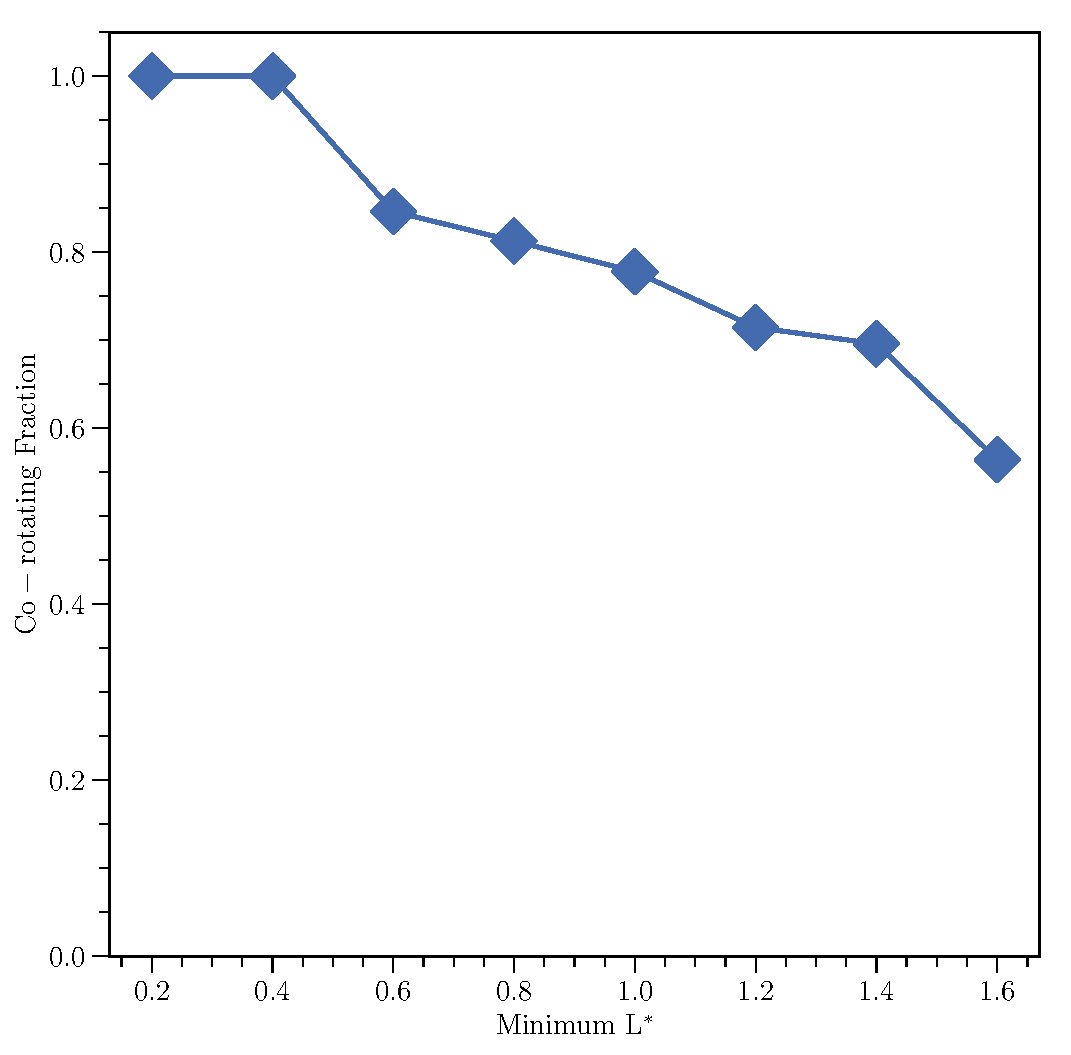
\includegraphics[width=0.49\textwidth]{SALT_corotate_vs_Lstar_minimum_velstrict_True_non_True_minsep_False.pdf}
        \caption{\small{The fraction of co-rotating absorbers as a function of minimum $L^{\**}$. All systems are included at $L^{\**}$=1.6 (this bin includes galaxies brighter than 1.6$L^{\**}$ as well), then only galaxies with $L^{\**} \leq 1.4$ are included at $L^{\**}$ =1.4, and so on.}}
%        \vspace{-5pt}
        \label{Lstar_fraction}
\end{figure}


\begin{figure}[ht!]
        \centering
        \vspace{0pt}
        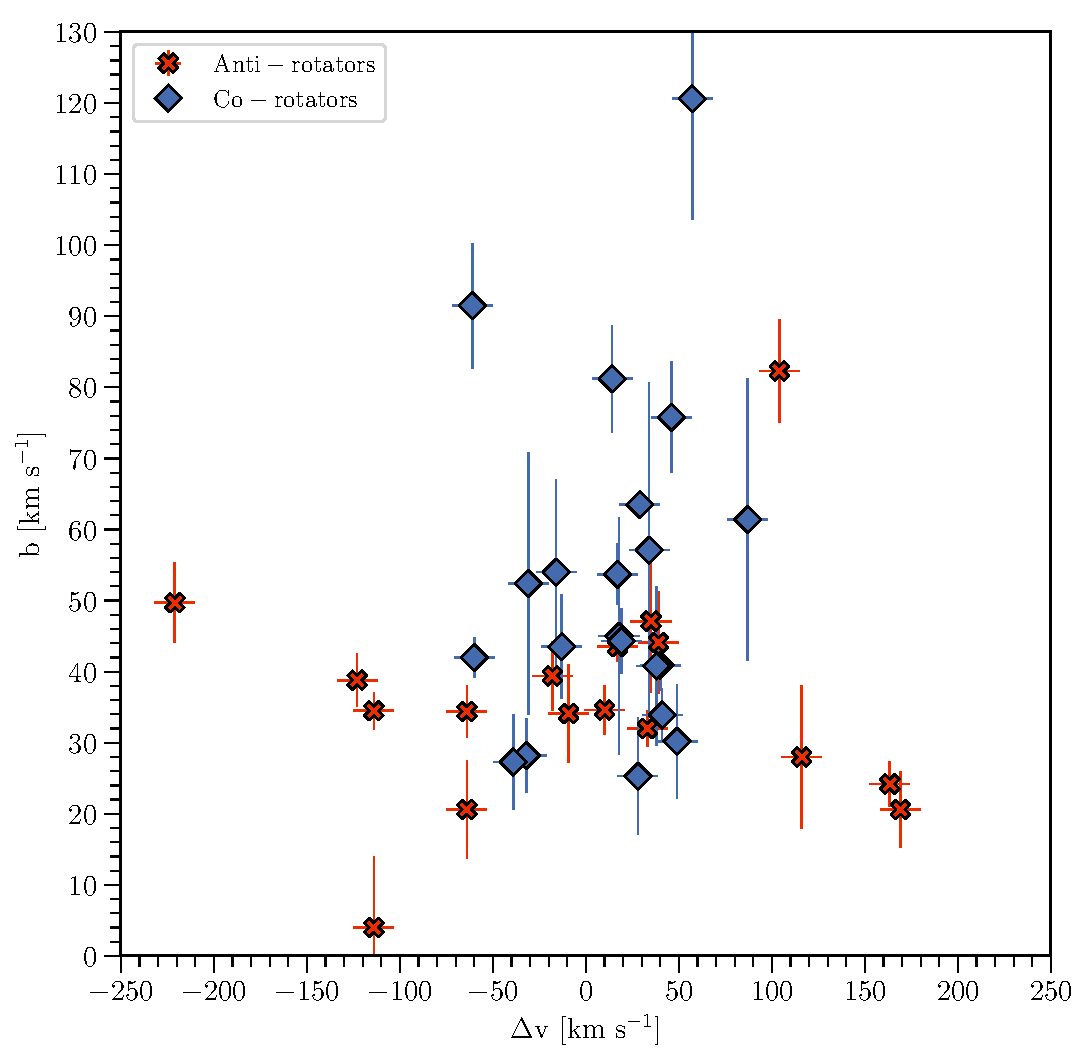
\includegraphics[width=0.49\textwidth]{SALT_b_vs_dv_velstrict_True_non_True_Lstar_0_5_minsep_False_fits_True.pdf}
        \caption{\small{The Doppler b-parameters of each absorber as a function of $\Delta v$, split into co-rotating (blue diamonds) and anti-rotating (red crosses). The data point for the NGC3067-3C232 LLS ($b = 245.2 \pm 25.9,  ~\Delta v = -68.0 \pm 11$ \kms) is not shown in order to highlight the majority distribution in greater detail.}}
%        \vspace{-5pt}
        \label{b_vs_dv}
\end{figure}





\begin{figure}[ht!]
        \centering
        \vspace{0pt}
        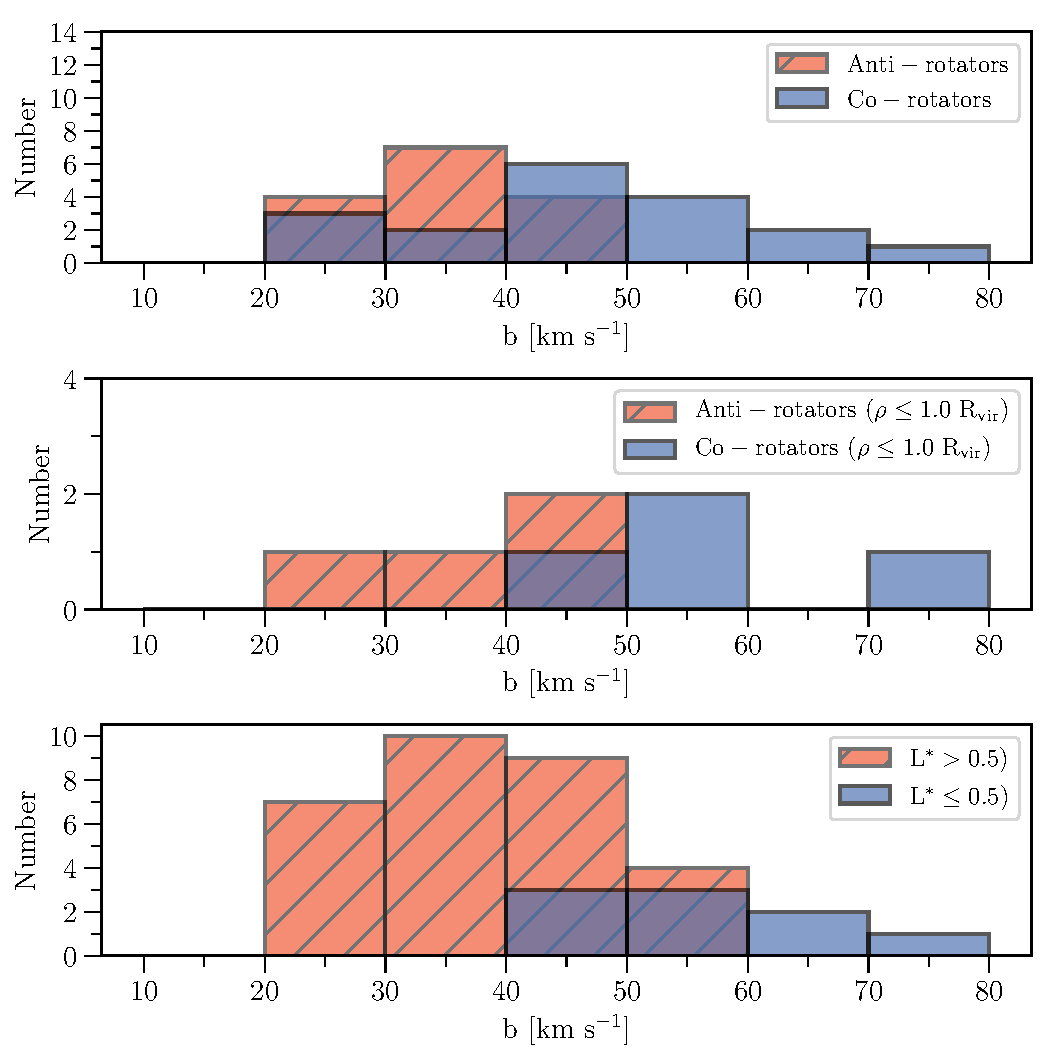
\includegraphics[width=0.45\textwidth]{SALT_bhist_velstrict_True_non_True_Lstar_0_5_minsep_False_fits_True.pdf}
        \caption{\small{Histograms showing the distributions of Doppler b-parameters for all Ly$\alpha$ absorbers with $V_{Ly\alpha} \leq V_{rot} \pm 10$ \kms. In the top panel we separate them into co-rotating (blue) and anti-rotating (red-hatched) subsets, in the middle we do the same but only for $\rho \leq 1 R_{vir}$, and on the bottom we separate based on absorbers near $L^{\**} \leq 0.5$ (blue) and $L^{\**} > 0.5$ (red-hatched) galaxies.}}
%        \vspace{-5pt}
        \label{b_hist}
\end{figure}


\begin{figure*}[ht!]
        \centering
        \vspace{0pt}
        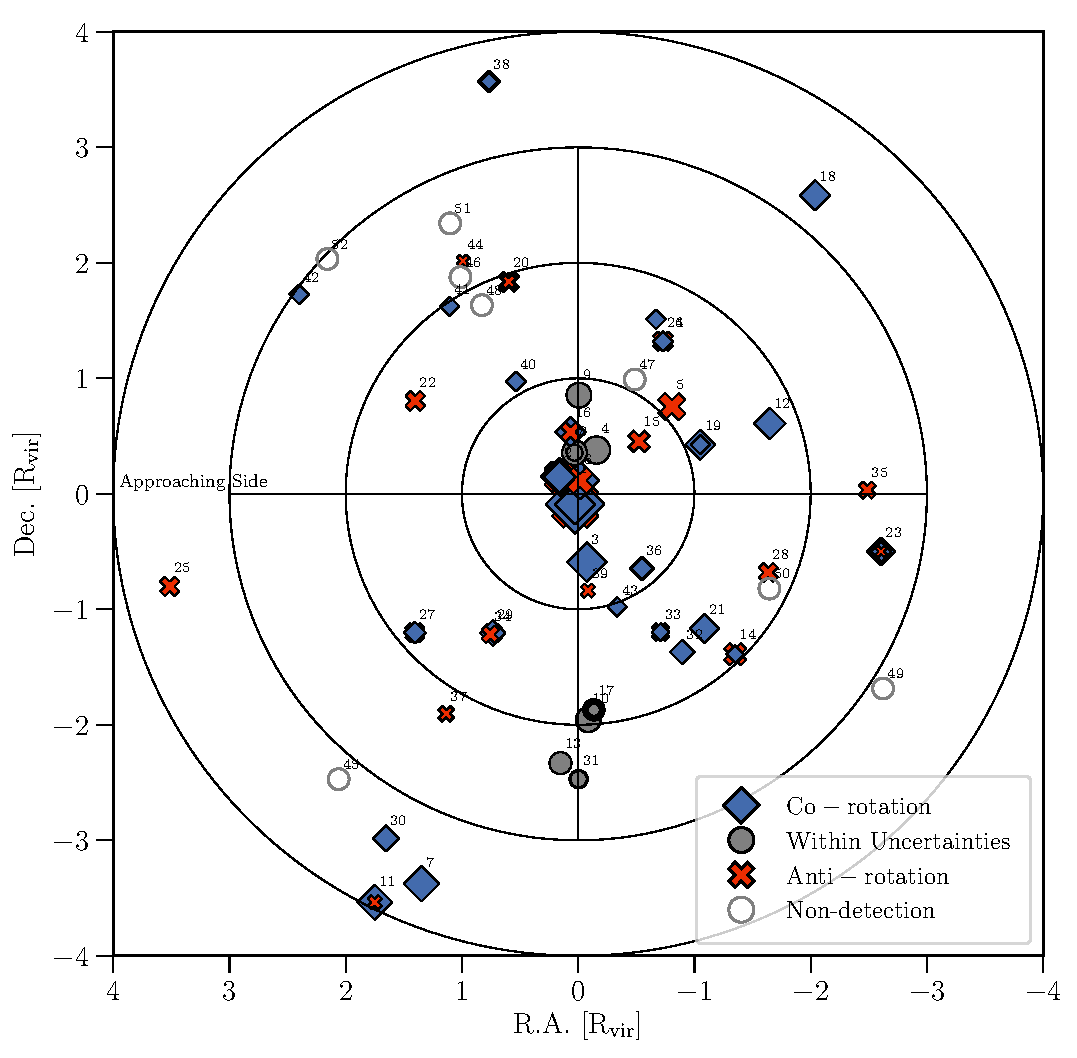
\includegraphics[width=0.95\textwidth]{SALTmap_velstrict_False_non_True_Lstar_0-100_minsep_False_azlim_85.pdf}
        \caption{\small{A map of the locations of each absorber normalized with respect to the galaxy virial radius. The color and style of each point indicates the line-of-sight velocity compared to that of the rotation of the nearby galaxy. Blue diamonds indicate co-rotation, red crosses indicate anti-rotation, and grey circles indicate cases where either is possible due to a combination of orientation and velocity uncertainties. The size of each point is scaled to reflect the EW of the absorber. Concentric rings indicate distances of 1, 2, 3 and 4 $R_{vir}$. All galaxies are rotated to PA = 90 or 270, such that their major axis' are horizontal and their approaching side is on the left as indicated. }}
%        \vspace{-5pt}
        \label{map}
\end{figure*}


\begin{figure}[ht!]
        \centering
        \vspace{0pt}
        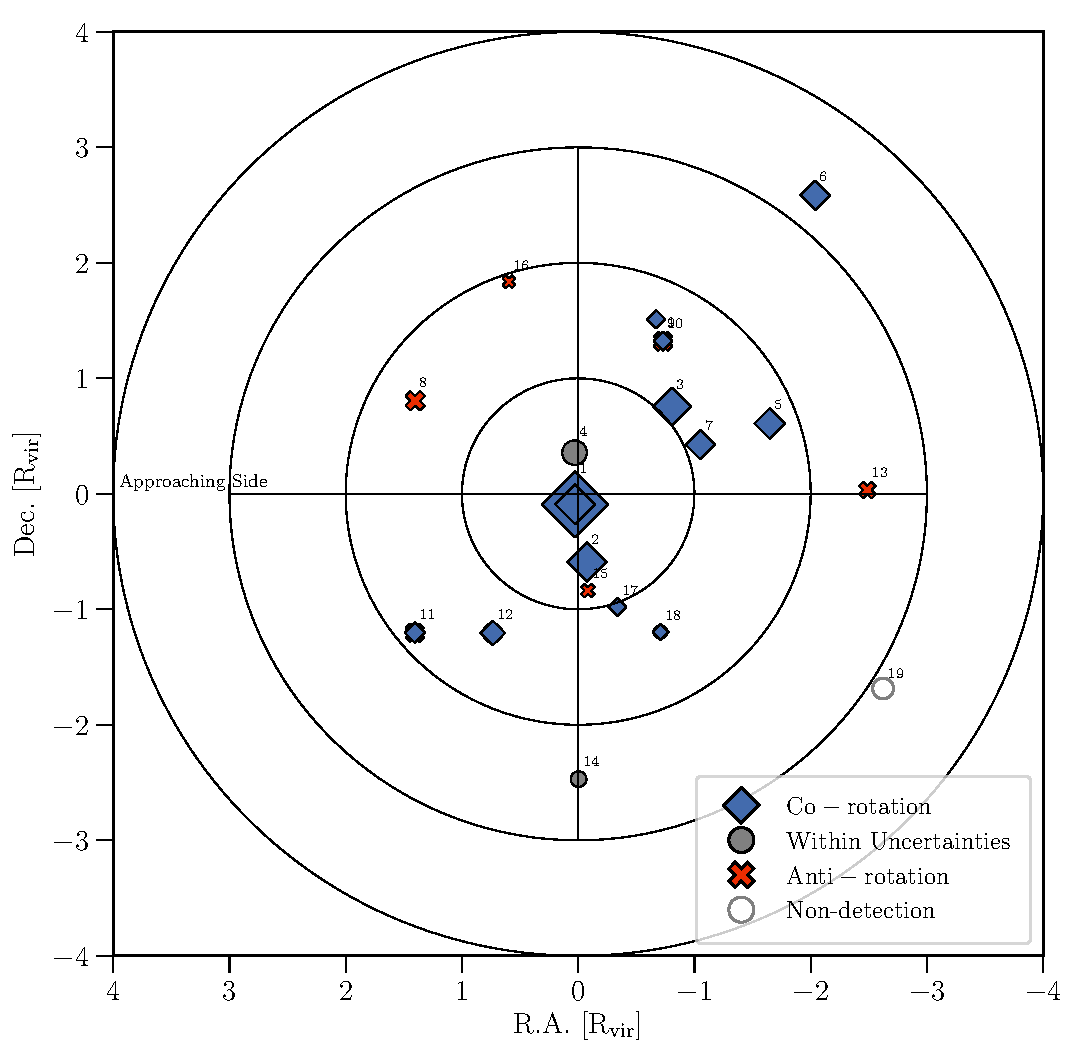
\includegraphics[width=0.48\textwidth]{SALTmap_NFW_model_velstrict_True_non_True_Lstar_0-100_minsep_20_azlim_85.pdf}
        \caption{\small{A map of the locations of each absorber normalized with respect to the galaxy virial radius. The color and style of each point indicates the NFW rotation model results for each absorber with $V_{Ly\alpha} \leq V_{rot}$ and 20 kpc nearest-neighbor constraints imposed. Blue diamonds indicate co-rotation, red crosses indicate anti-rotation, and grey circles indicate cases where either is possible due to a combination of orientation and velocity uncertainties. The size of each point is scaled to reflect the EW of the absorber. Concentric rings indicate distances of 1, 2, 3 and 4 $R_{vir}$. All galaxies are rotated to PA = 90 or 270, such that their major axis' are horizontal and their approaching side is on the left as indicated.}}
%        \vspace{-5pt}
        \label{map}
\end{figure}


\begin{figure}[ht!]
        \centering
        \vspace{0pt}
        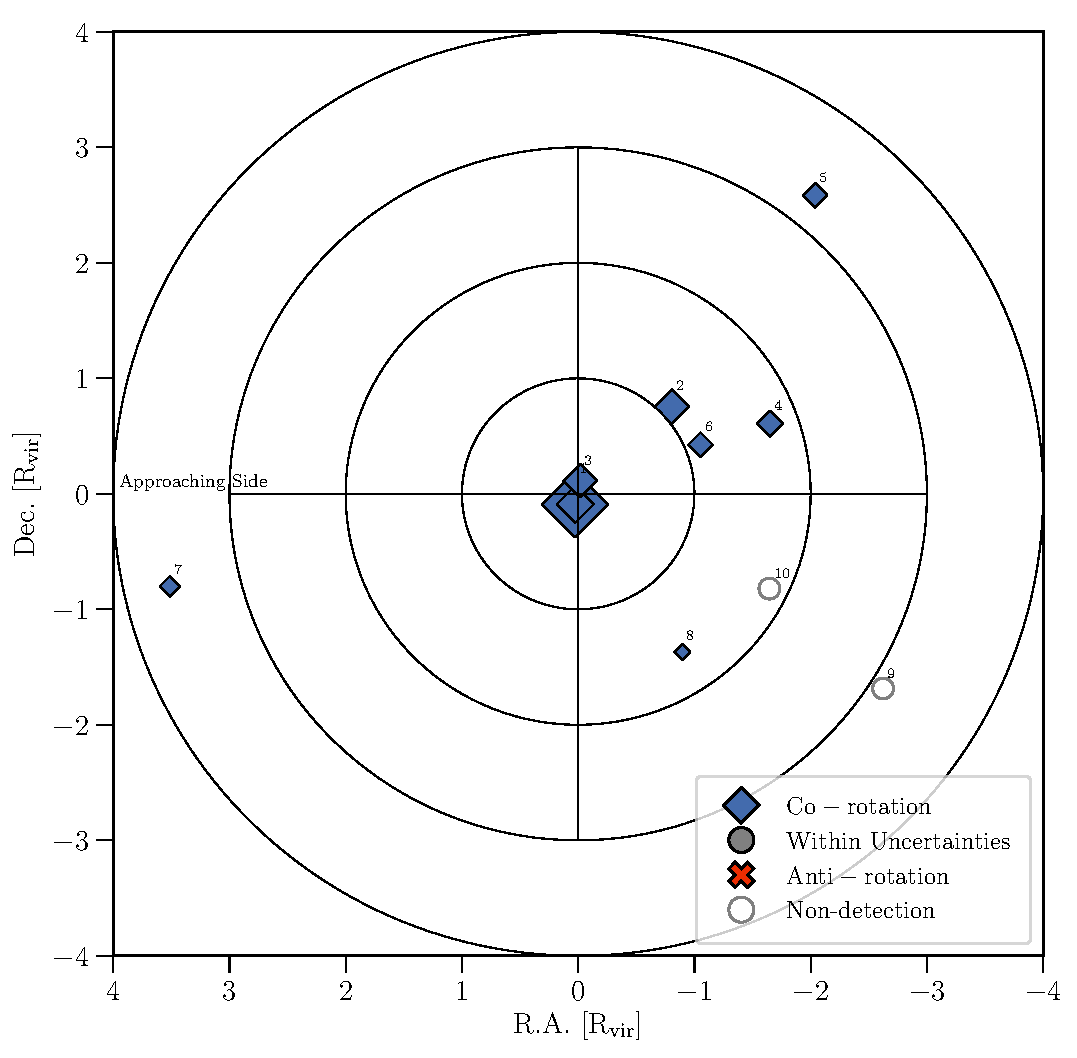
\includegraphics[width=0.48\textwidth]{SALTmap_NFW_model_velstrict_True_non_True_Lstar_0-0_5_minsep_False_azlim_85.pdf}
        \caption{\small{A map of the locations of each absorber normalized with respect to the galaxy virial radius. The color and style of each point indicates the NFW rotation model results for each absorber with $V_{Ly\alpha} \leq V_{rot}$ and $[L^{\**} > 0.5]$ constraints imposed. Blue diamonds indicate co-rotation, red crosses indicate anti-rotation, and grey circles indicate cases where either is possible due to a combination of orientation and velocity uncertainties. The size of each point is scaled to reflect the EW of the absorber. Concentric rings indicate distances of 1, 2, 3 and 4 $R_{vir}$. All galaxies are rotated to PA = 90 or 270, such that their major axis' are horizontal and their approaching side is on the left as indicated. }}
%        \vspace{-5pt}
        \label{map}
\end{figure}


%\begin{figure}[t!]
%\centering
%  \subfigure[]{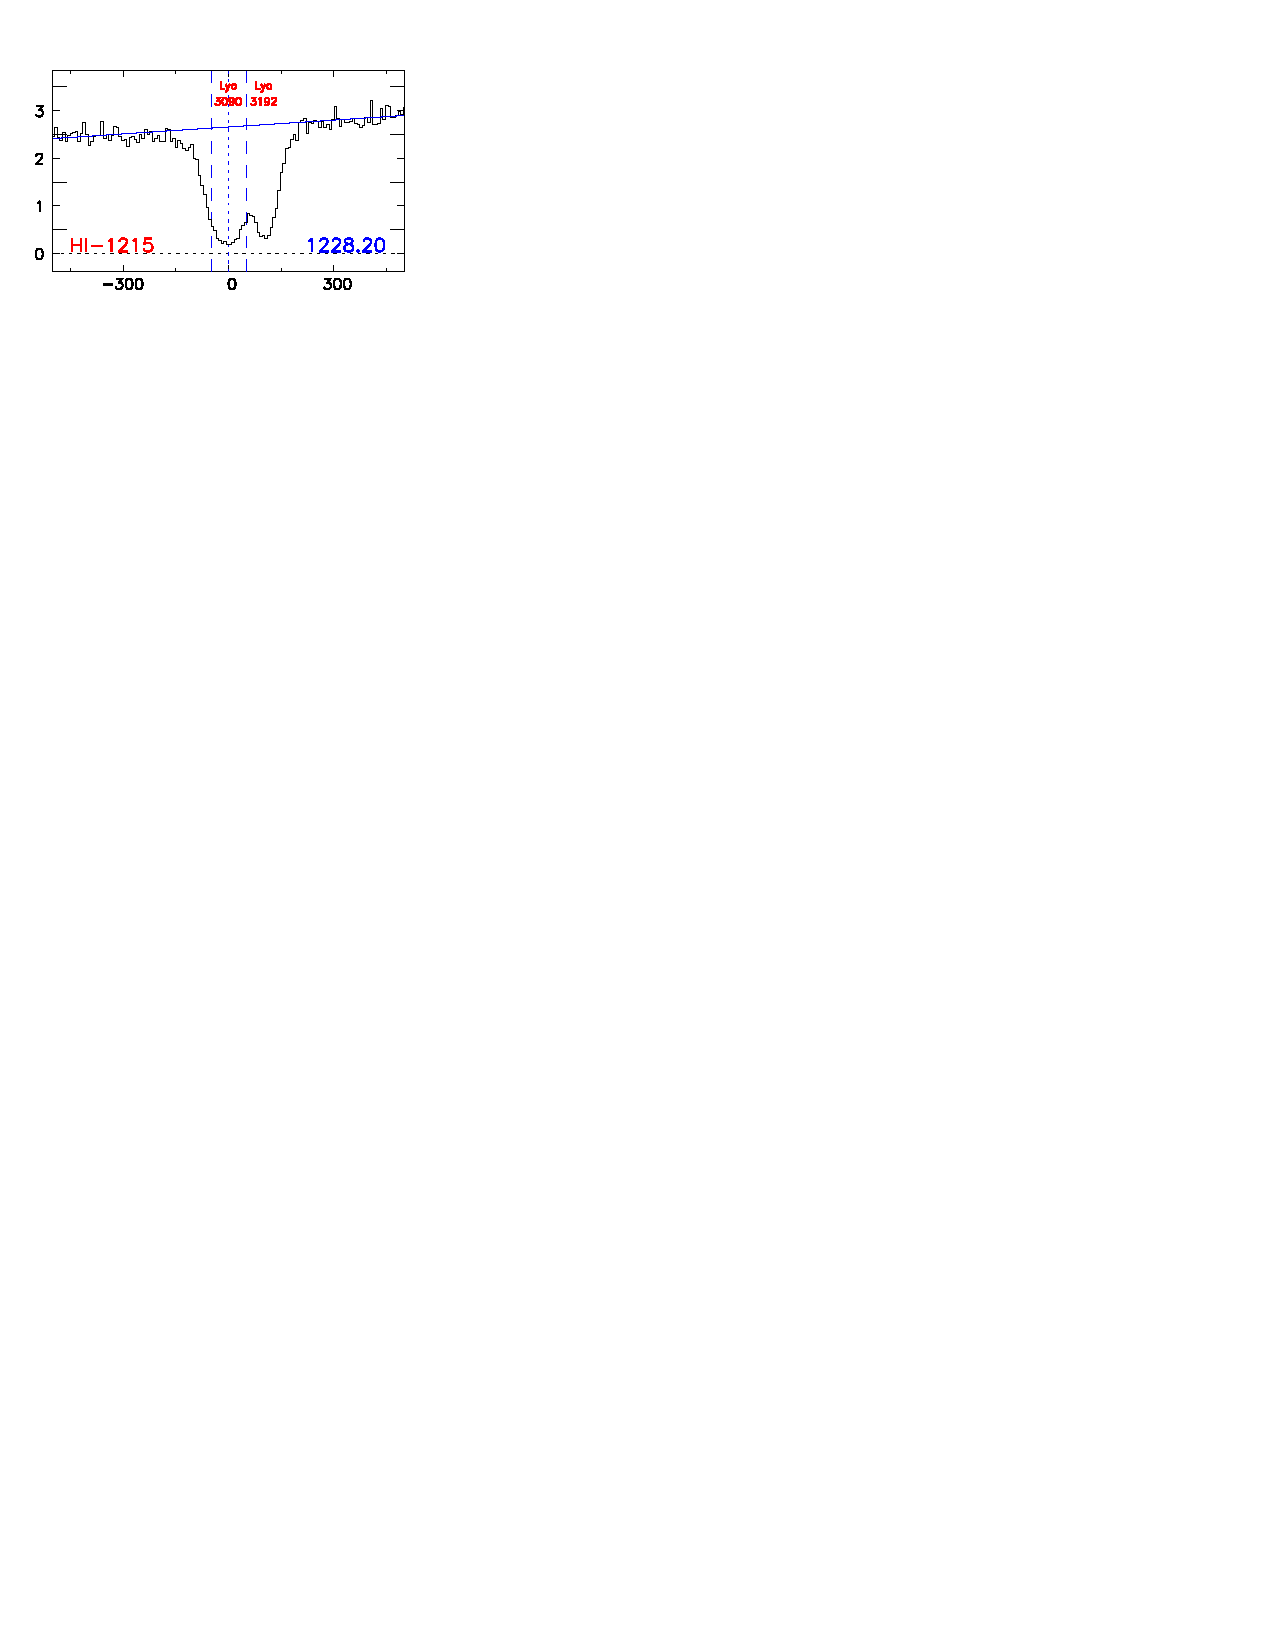
\includegraphics[width=0.87\linewidth]{fig2.pdf}}{\label{line}}
%  \subfigure[]{\includegraphics[width=1.\linewidth]{fig3.pdf}\label{impactmap}}
%  \caption{\small{a) An example of 2 Ly$\alpha$ lines found in the Mrk290 sightline at 3090 and 3192 . b) A map of \textit{all} galaxies within a 500 kpc impact parameter of target Mrk290 sightline and with velocity ($cz$) within 400 $\rm km\, s^{-1}$ of absorption detected at 3192 $\rm km\, s^{-1}$ (central black star). The galaxy NGC5987 ($v=3010$ $\rm km\, s^{-1}$, inclination = $65^{\circ}$) can be unambiguously paired with the Ly$\alpha$ absorption features at $v=3090, 3192$ $\rm km\, s^{-1}$ because it is the largest and closest galaxy in both physical and velocity space to the absorption feature.}}
%\vspace{5pt}
%\end{figure}




\section{Summary}

\section{Sightlines needed}
The following targets need to be added: \\
SBS1304+594 \\
SDSSJ112632.90+120437.0 \\
SDSSJ112756.70+115427.0 \\
RX\_J1054.2+3511 - check for feature around 600 \kms \\
MS1047.3+3518 \\
%TON1009 \\
%SDSSJ095914.80+320357.0 \\
RX\_J1002.9+3240 \\
%RX\_J1142.7+4625 \\
SDSSJ152053.59+571122.1 \\
SDSSJ104816.30+120735.0 \\
SDSSJ104709.80+130454.0 \\
SDSSJ104843.50+130605.0 \\
SDSSJ105220.60+101751.0 \\
SDSSJ104341.53+085558.2 \\
SDSSJ101622.60+470643.0 \\


%\begin{table}[ht]\footnotesize
%\begin{center}
%\begin{tabular}{l l l}
% \hline \hline
% Statistic                				&  Blueshifted Absorbers   &     Redshifted Absorbers     \\ 
%  \hline \hline
% Number 	          			 		&     	22				&	26			\\
% Mean $EW$    \scriptsize $\rm [m\AA]$    &	$329 \pm 52$ 		&	$245 \pm 34$  	\\
%  
%\hline
%\end{tabular}
%\end{center}
%  \caption{\small{Average properties of the associated galaxy sample split into red and blue-shifted bins based on $\Delta v$.}}
%  \label{resultsTable}
%\end{table}


\vspace{10pt}


\acknowledgements

D. M. F. thanks Claire Murray for useful insights on our halo model, and Julie Davis for invaluable SALT data reduction pointers. This research has made use of the NASA/IPAC Extragalactic Database (NED) which is operated by the Jet Propulsion Laboratory, California Institute of Technology, under contract with the National Aeronautics and Space Administration. Based on observations with the NASA/ESA \textit{Hubble Space Telescope}, obtained at the Space Telescope Science Institute (STScI), which is operated by the Association of Universities for Research in Astronomy, Inc., under NASA contract NAS 5-26555. \textbf{SALT ACKNOWLEDGEMENT}. Spectra were retrieved from the Barbara A. Mikulski Archive for Space Telescopes (MAST) at STScI. Over the course of this study, D.M.F. and B.P.W. were supported by grant AST-1108913, awarded by the US National Science Foundation, and by NASA grants \textit{HST}-AR-12842.01-A, \textit{HST}-AR-13893.01-A, and \textit{HST}-GO-14240 (STScI). 

\facility{HST (COS), SALT (RSS)}
\clearpage

%\nocite{*}
%\bibliography{rotation_bib}
\bibliography{/Users/frenchd/Research/bib}{}
\bibliographystyle{apj}

\clearpage

\appendix

\section{Rotation Curves}
\label{rotation_curves}
Here we present rotation curves with finder charts indicating the slit position for each galaxy observed with SALT. 

\begin{figure}[h]
\centering
  \subfigure[]{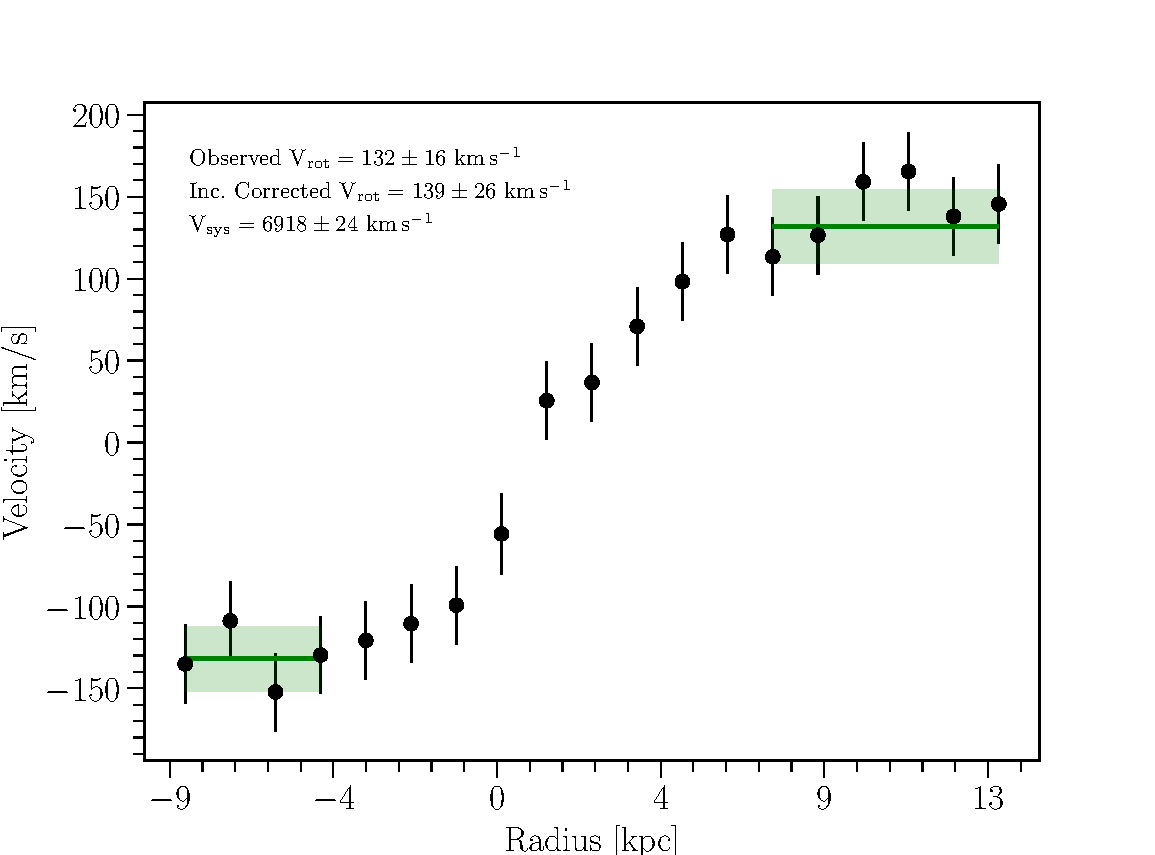
\includegraphics[width=.54\linewidth]{CGCG039-137_2_rotation_curve_xphys_helio_vobs_vrotObs_new4.pdf}}{\label{rotationcurve_CGCG039-137}}
  \subfigure[]{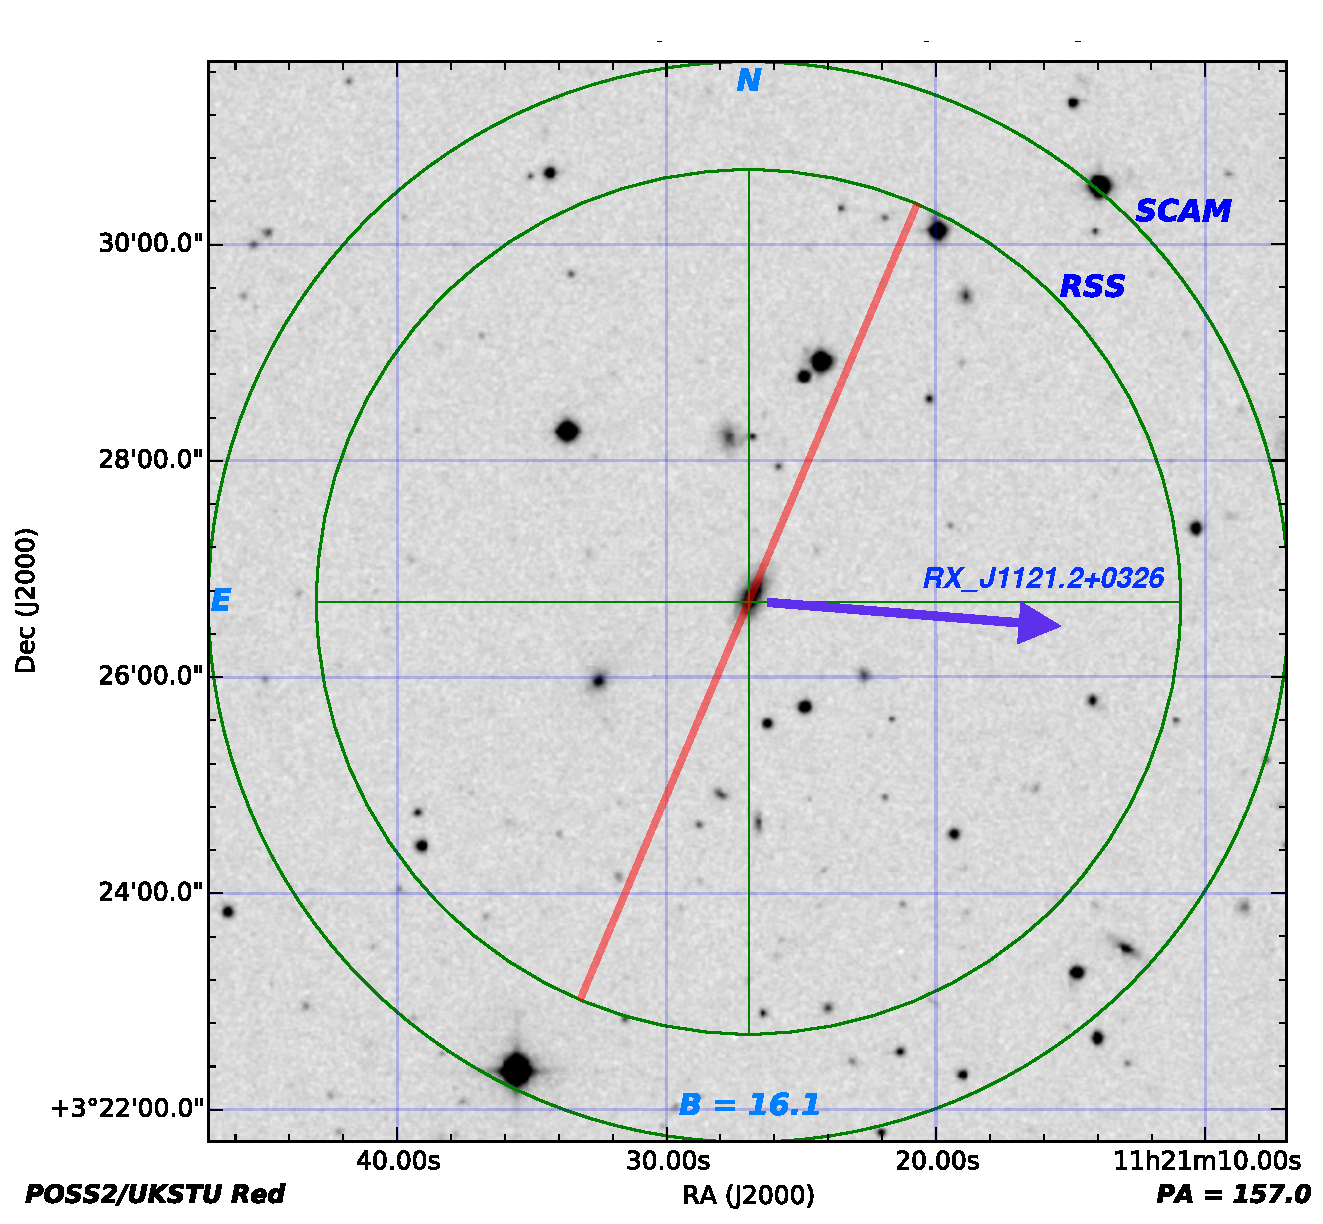
\includegraphics[width=0.45\linewidth]{CGCG039-137_Finding_chart.pdf}\label{finderchart_CGCG039-137}}
  \caption{\small{a) Rotation curve of CGCG039-137. The solid green line indicates the weighted mean velocity over the corresponding x-axis region, and the shaded green indicates the 1$\sigma$ error in the mean. b) SALT finder chart for CGCG039-137 showing the position of the slit in red.}}
\vspace{0pt}
\end{figure}


\begin{figure}[h]
\centering
  \subfigure[]{\includegraphics[width=.54\linewidth]{IC5325_2_rotation_curve_xphys_helio_vobs_vrotObs_new4.pdf}}{\label{rotationcurve_IC5325}}
  \subfigure[]{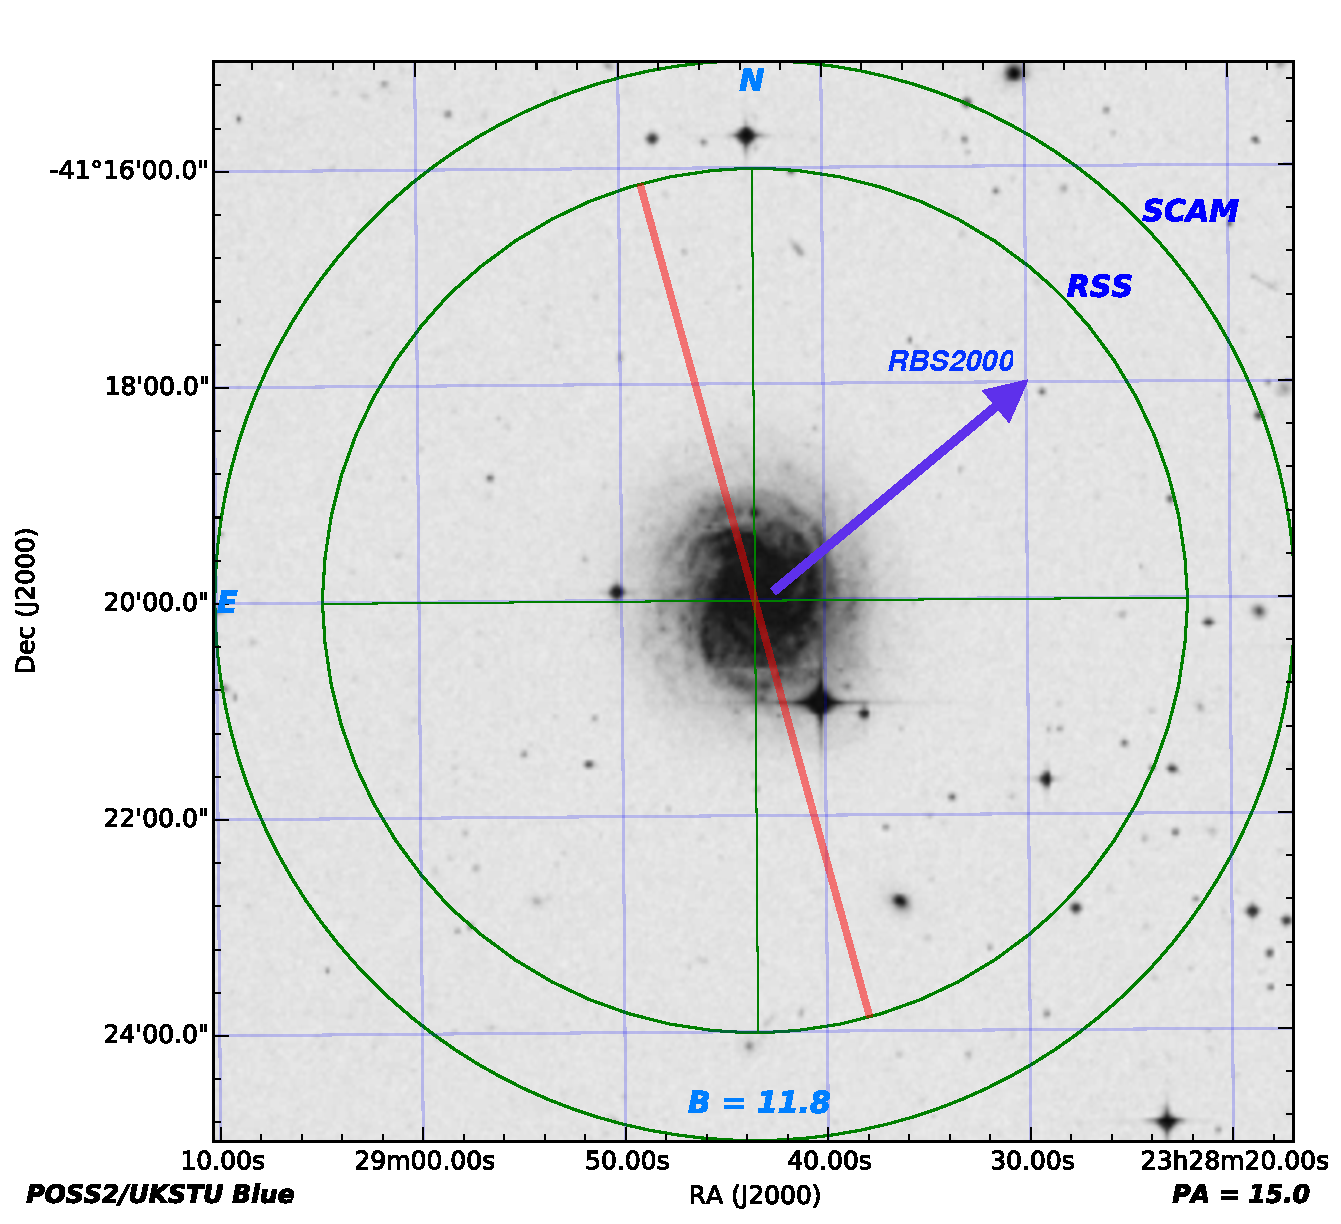
\includegraphics[width=0.45\linewidth]{IC5325_FindingChart.pdf}\label{finderchart_IC5325}}
  \caption{\small{a) Rotation curve of IC5325. The solid green line indicates the weighted mean velocity over the corresponding x-axis region, and the shaded green indicates the 1$\sigma$ error in the mean. b) SALT finder chart for IC5325 showing the position of the slit in red.}}
\vspace{0pt}
\end{figure}


\begin{figure}[t!]
\centering
  \subfigure[]{\includegraphics[width=.54\linewidth]{MCG-03-58-009_2_rotation_curve_xphys_helio_vobs_vrotObs_new4.pdf}}{\label{rotationcurve_MCG-03-58-009}}
  \subfigure[]{\includegraphics[width=0.45\linewidth]{MCG-03-58-009_FindingChart.pdf}\label{finderchart_MCG-03-58-009}}
  \caption{\small{a) Rotation curve of MCG-03-58-009. The solid green line indicates the weighted mean velocity over the corresponding x-axis region, and the shaded green indicates the 1$\sigma$ error in the mean. b) SALT finder chart for MCG-03-58-009 showing the position of the slit in red.}}
\vspace{0pt}
\end{figure}


\begin{figure}[h]
\centering
  \subfigure[]{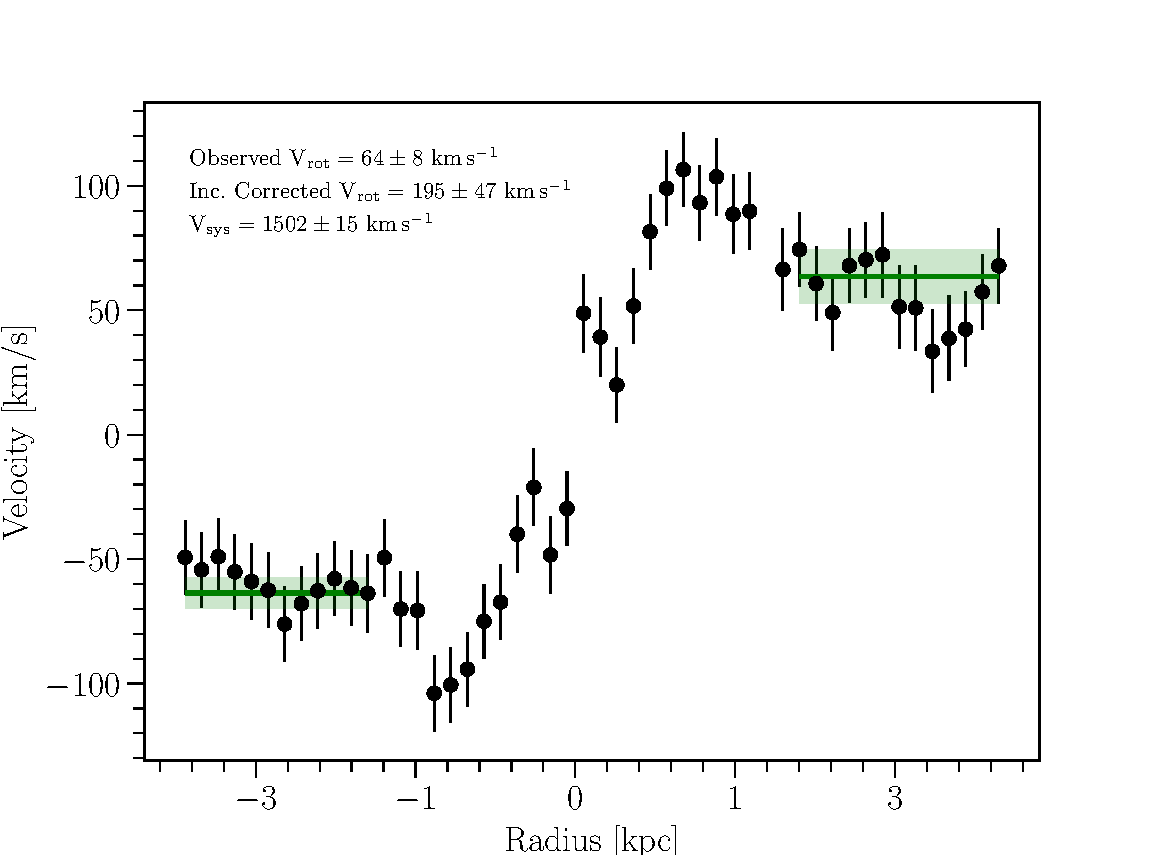
\includegraphics[width=.54\linewidth]{NGC1566_2_rotation_curve_xphys_helio_vobs_vrotObs_new4.pdf}}{\label{rotationcurve_NGC1566}}
  \subfigure[]{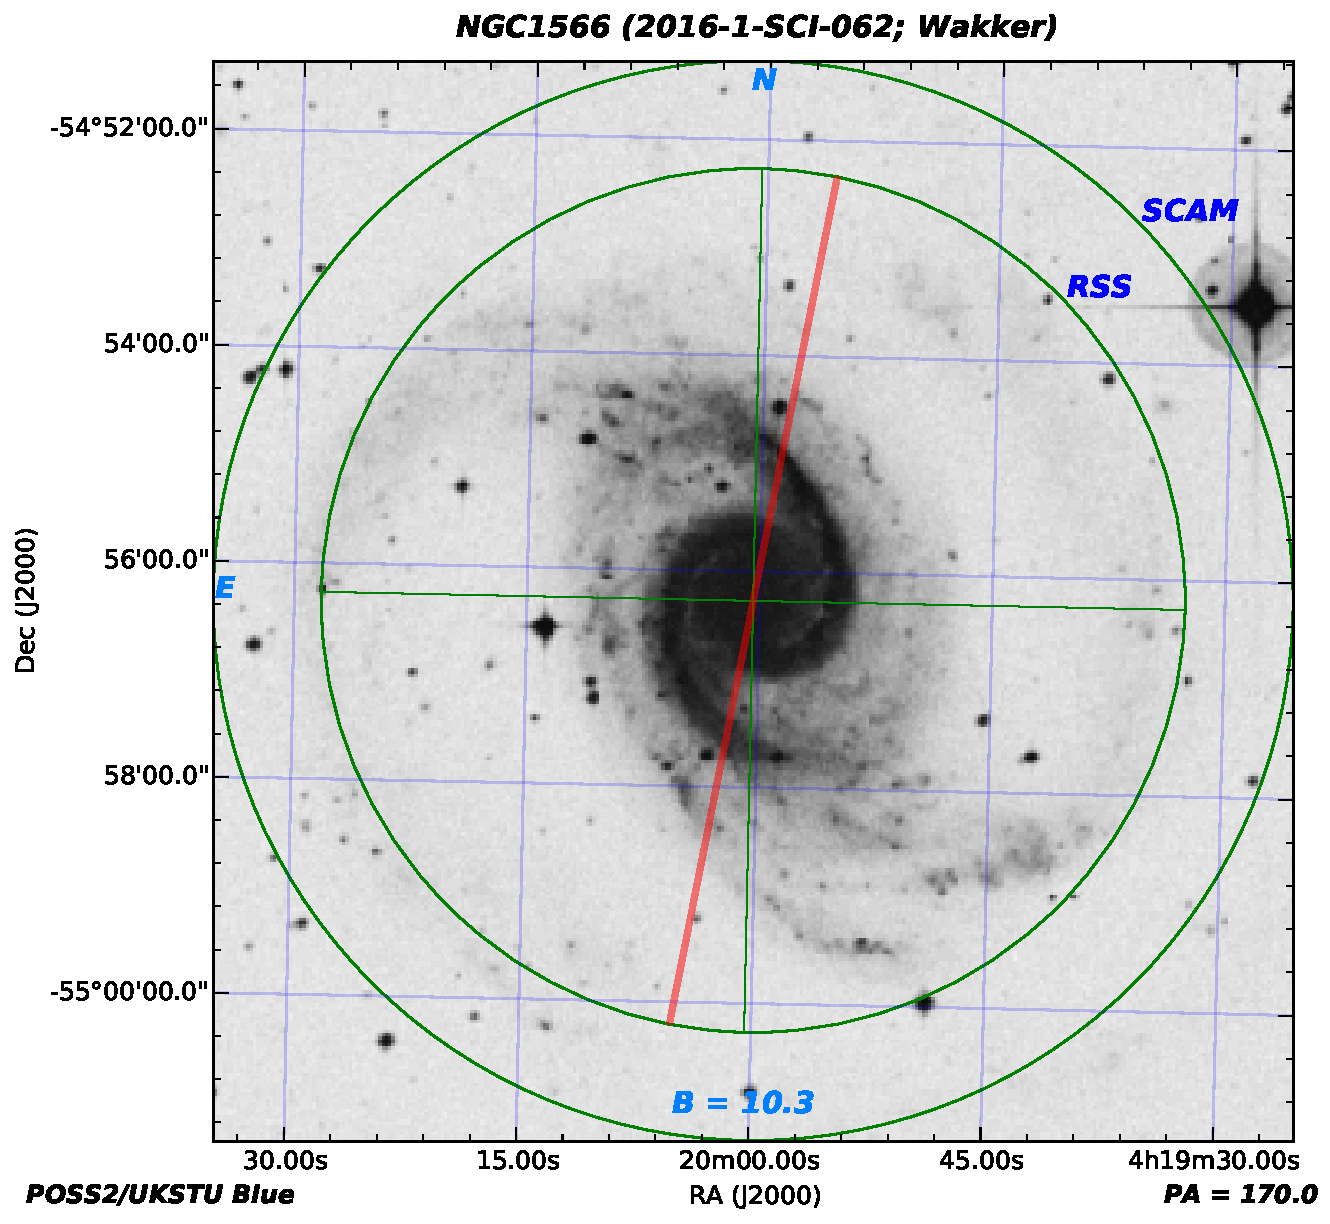
\includegraphics[width=0.45\linewidth]{NGC1566_FindingChart.pdf}\label{finderchart_NGC1566}}
  \caption{\small{a) Rotation curve of NGC1566. The solid green line indicates the weighted mean velocity over the corresponding x-axis region, and the shaded green indicates the 1$\sigma$ error in the mean. b) SALT finder chart for NGC1566 showing the position of the slit in red.}}
\vspace{0pt}
\end{figure}


\begin{figure}[h]
\centering
  \subfigure[]{\includegraphics[width=.54\linewidth]{NGC3513_2_rotation_curve_xphys_helio_vobs_vrotObs_new4.pdf}}{\label{rotationcurve_NGC3513}}
  \subfigure[]{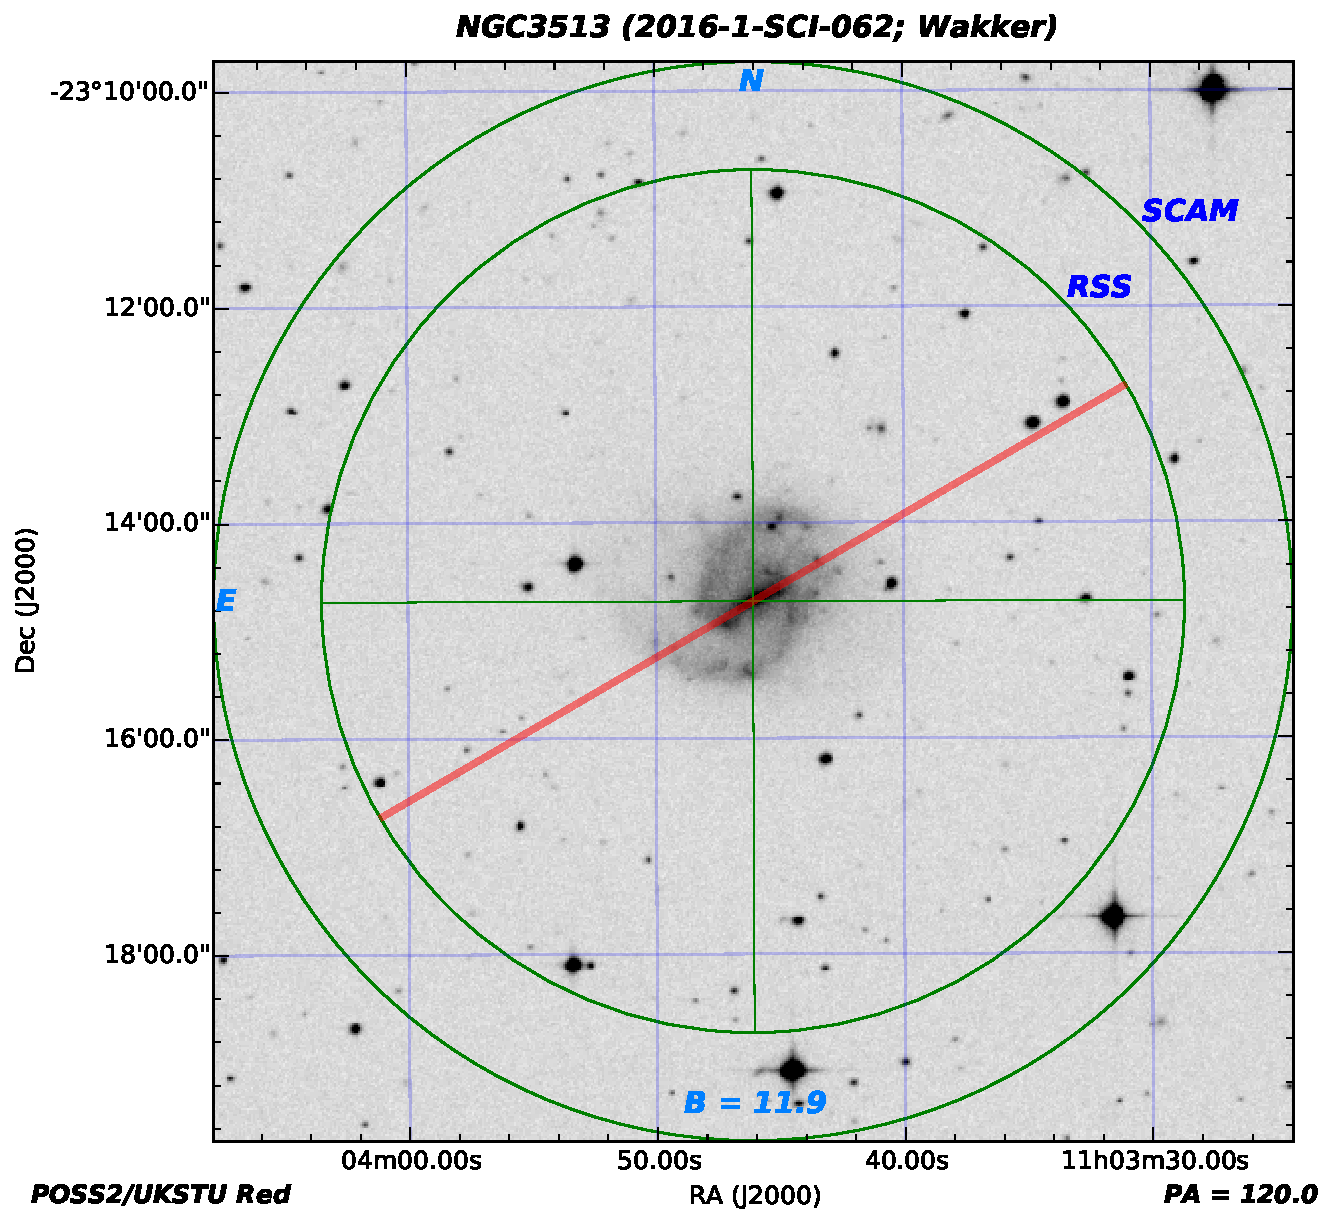
\includegraphics[width=0.45\linewidth]{NGC3513_Finding_chart.pdf}\label{finderchart_NGC3513}}
  \caption{\small{a) Rotation curve of NGC3513. The solid green line indicates the weighted mean velocity over the corresponding x-axis region, and the shaded green indicates the 1$\sigma$ error in the mean. b) SALT finder chart for NGC3513 showing the position of the slit in red.}}
\vspace{0pt}
\end{figure}


\begin{figure}[h]
\centering
  \subfigure[]{\includegraphics[width=.54\linewidth]{NGC3633_2_rotation_curve_xphys_helio_vobs_vrotObs_new4.pdf}}{\label{rotationcurve_NGC3633}}
  \subfigure[]{\includegraphics[width=0.45\linewidth]{NGC3633_FindingChart.pdf}\label{finderchart_NGC3633}}
  \caption{\small{a) Rotation curve of NGC4536. The solid green line indicates the weighted mean velocity over the corresponding x-axis region, and the shaded green indicates the 1$\sigma$ error in the mean. b) SALT finder chart for NGC3633 showing the position of the slit in red.}}
\vspace{0pt}
\end{figure}


\begin{figure}[h]
\centering
  \subfigure[]{\includegraphics[width=.54\linewidth]{NGC4536_2_rotation_curve_xphys_helio_vobs_vrotObs_new4.pdf}}{\label{rotationcurve_NGC4536}}
  \subfigure[]{\includegraphics[width=0.45\linewidth]{NGC4536_FindingChart.pdf}\label{finderchart_NGC4536}}
  \caption{\small{a) Rotation curve of NGC4536. The solid green line indicates the weighted mean velocity over the corresponding x-axis region, and the shaded green indicates the 1$\sigma$ error in the mean. b) SALT finder chart for NGC4536 showing the position of the slit in red.}}
\vspace{0pt}
\end{figure}


\begin{figure}[h]
\centering
  \subfigure[]{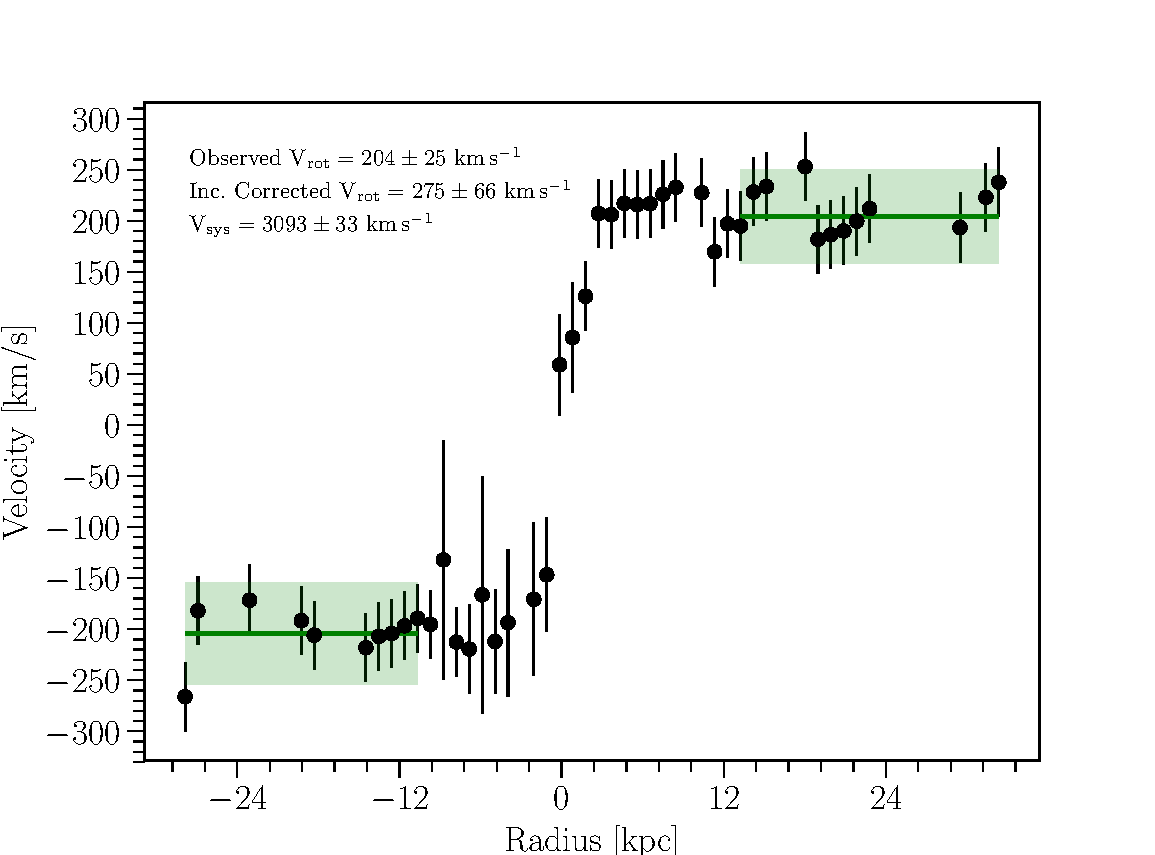
\includegraphics[width=.54\linewidth]{NGC4939_2_rotation_curve_xphys_helio_vobs_vrotObs_new4.pdf}}{\label{rotationcurve_NGC4939}}
  \subfigure[]{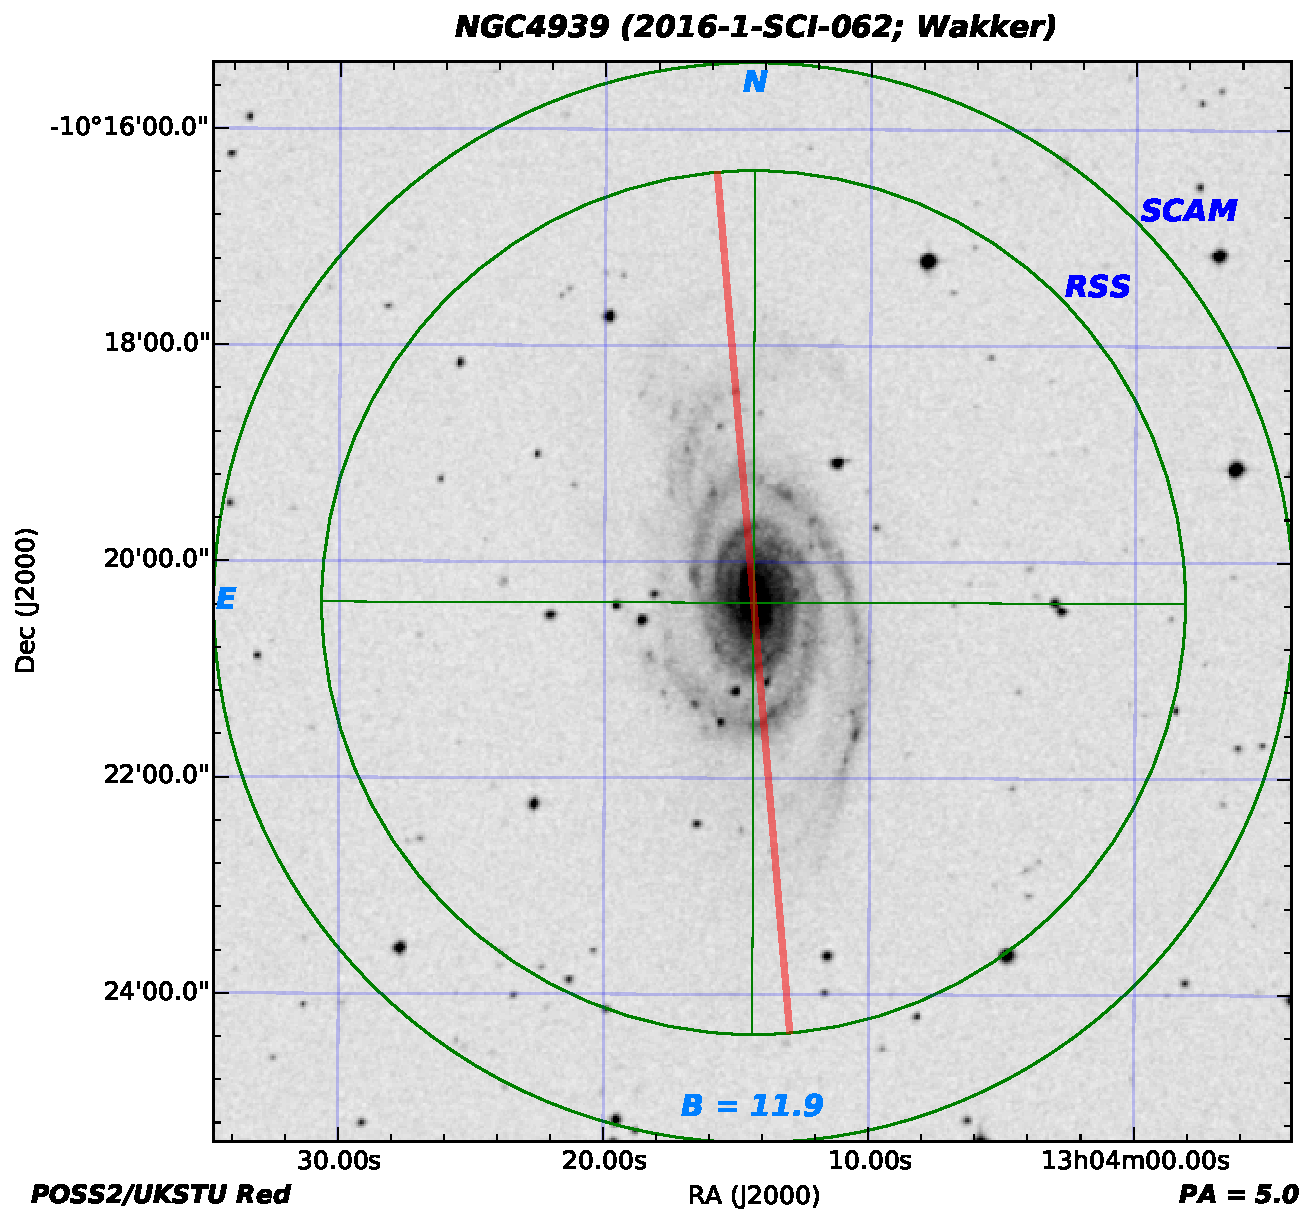
\includegraphics[width=0.45\linewidth]{NGC4939_FindingChart.pdf}\label{finderchart_NGC4939}}
  \caption{\small{a) Rotation curve of NGC4939. The solid green line indicates the weighted mean velocity over the corresponding x-axis region, and the shaded green indicates the 1$\sigma$ error in the mean. b) SALT finder chart for NGC4939 showing the position of the slit in red.}}
\vspace{0pt}
\end{figure}


\begin{figure}[h]
\centering
  \subfigure[]{\includegraphics[width=.54\linewidth]{NGC5364_2_rotation_curve_xphys_helio_vobs_vrotObs_new4.pdf}}{\label{rotationcurve_NGC5364}}
  \subfigure[]{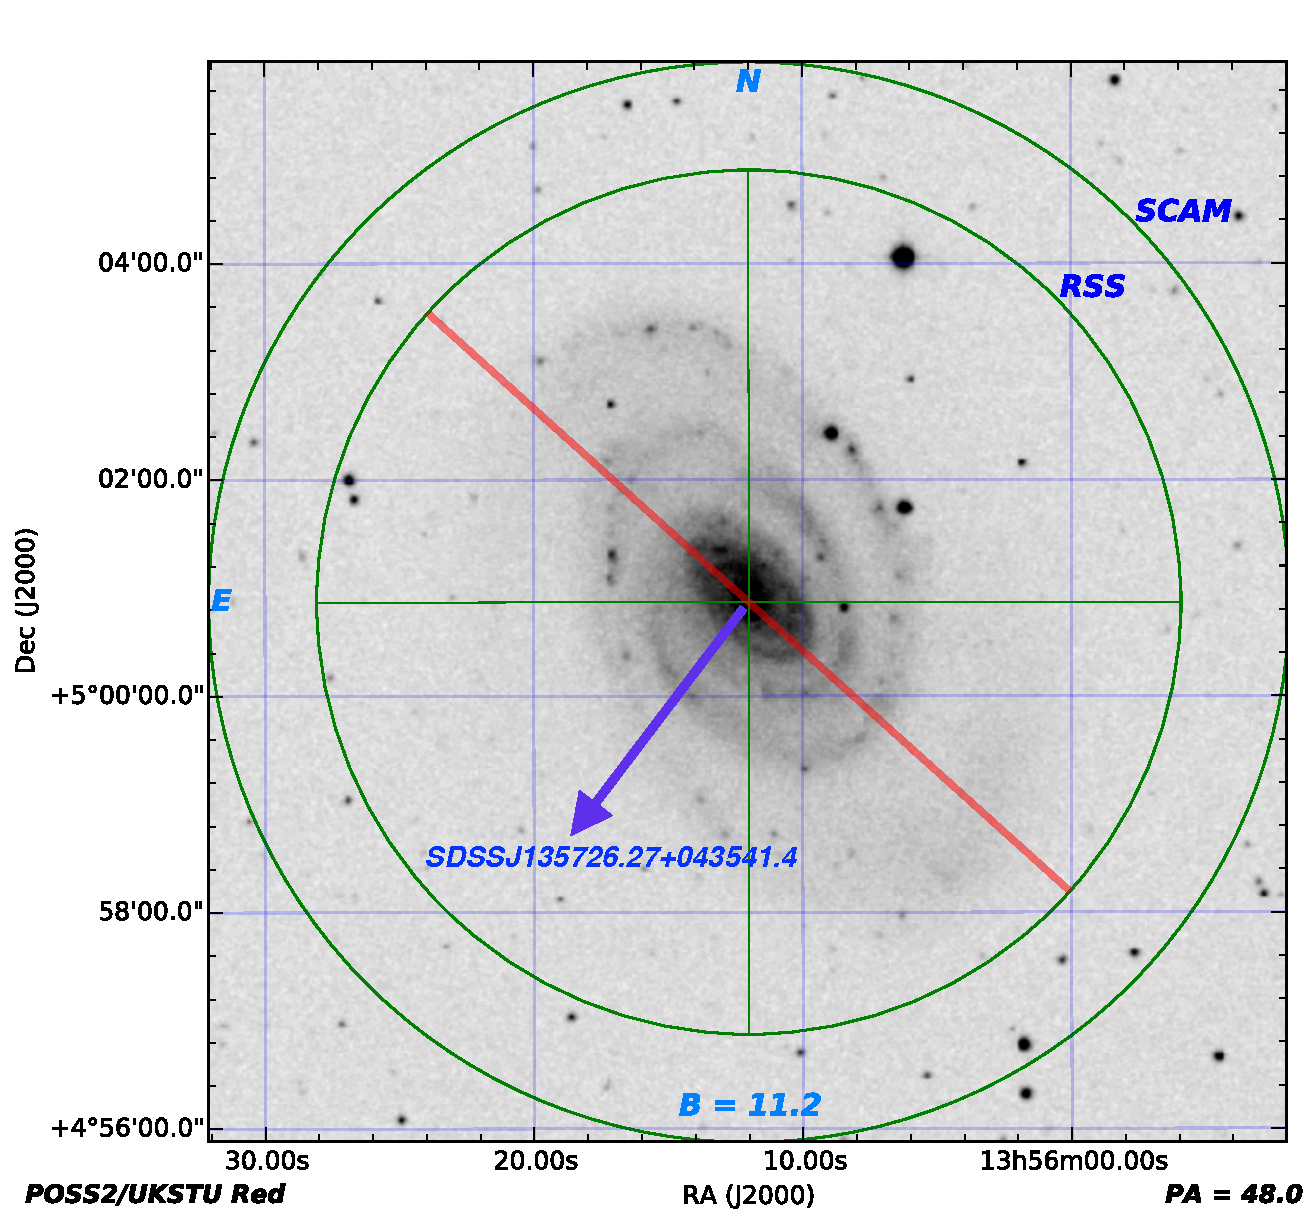
\includegraphics[width=0.45\linewidth]{NGC5364_FindingChart.pdf}\label{finderchart_NGC5364}}
  \caption{\small{a) Rotation curve of NGC5364. The solid green line indicates the weighted mean velocity over the corresponding x-axis region, and the shaded green indicates the 1$\sigma$ error in the mean. b) SALT finder chart for NGC5364 showing the position of the slit in red.}}
\vspace{0pt}
\end{figure}


\begin{figure}[h]
\centering
  \subfigure[]{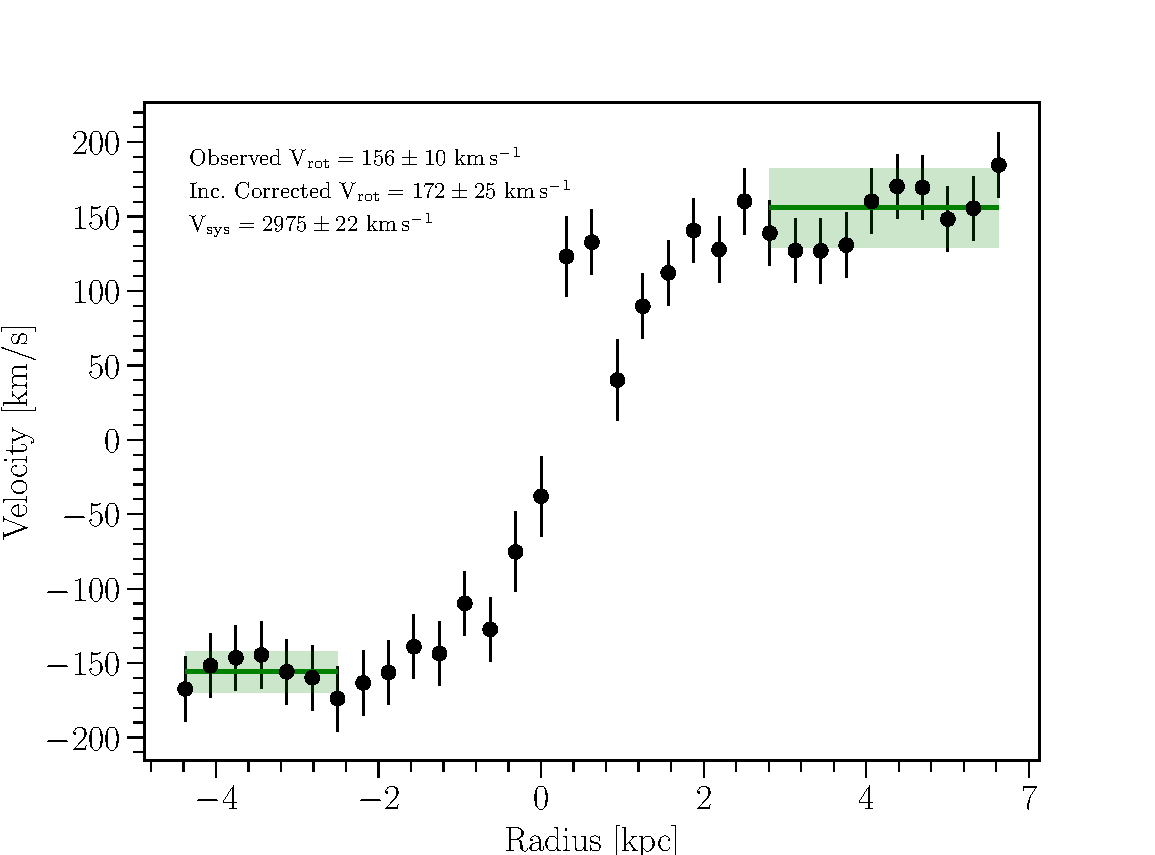
\includegraphics[width=.54\linewidth]{NGC5786_2_rotation_curve_xphys_helio_vobs_vrotObs_new4.pdf}}{\label{rotationcurve_NGC5786}}
  \subfigure[]{\includegraphics[width=0.45\linewidth]{NGC5786_FindingChart.pdf}\label{finderchart_NGC5786}}
  \caption{\small{a) Rotation curve of NGC5786. The solid green line indicates the weighted mean velocity over the corresponding x-axis region, and the shaded green indicates the 1$\sigma$ error in the mean. b) SALT finder chart for NGC5786 showing the position of the slit in red.}}
\vspace{0pt}
\end{figure}


\begin{figure}[h]
\centering
  \subfigure[]{\includegraphics[width=.54\linewidth]{RFGC3781_2_rotation_curve_xphys_helio_vobs_vrotObs_new4.pdf}}{\label{rotationcurve_RFGC3781}}
  \subfigure[]{\includegraphics[width=0.45\linewidth]{RFGC3781_FindingChart.pdf}\label{finderchart_RFGC3781}}
  \caption{\small{a) Rotation curve of NGC5364. The solid green line indicates the weighted mean velocity over the corresponding x-axis region, and the shaded green indicates the 1$\sigma$ error in the mean. b) SALT finder chart for NGC5364 showing the position of the slit in red.}}
\vspace{0pt}
\end{figure}


\end{document}
